% We use babel english for english acronyms with the acro package
\documentclass[english,spanish,a4paper,11pt]{article}
\usepackage[T1]{fontenc}
\usepackage{hyperref}
\usepackage[svgnames]{xcolor}

\usepackage{acro}
%\usepackage{acronym}
\usepackage{amsmath}
\usepackage{authblk}
\usepackage[es-noquoting,es-nodecimaldot,es-tabla]{babel}
\usepackage[alldates=comp,sorting=none,style=numeric-comp]{biblatex}
\usepackage{booktabs}
\usepackage{caption}
\usepackage{csquotes}
\usepackage{etoolbox}
\usepackage{graphicx}
\usepackage{listingsutf8}
\usepackage{microtype}
\usepackage{menukeys}
\usepackage{pgfplots}
\usepackage{siunitx}
\usepackage{tcolorbox}
\usepackage{varwidth}

\usepackage{cleveref}


% IBM Plex fonts
\usepackage{plex-serif}
\usepackage{plex-sans}
\usepackage{plex-mono}
\renewcommand*\familydefault{\sfdefault}


% pgfplots configuration
\pgfplotsset{compat=1.18}


% tcolobox libraries
\tcbuselibrary{
    breakable,
    hooks,
    listingsutf8,
    skins
}


% tikz libraries
\usetikzlibrary{
    arrows.meta,
    calc,
    decorations.pathmorphing,
    fit,
    positioning
}


% biblatex
\addbibresource{references.bib}

% siunitx configuration
\sisetup{detect-all}


% acro settings
\acsetup{
    locale/display=true,
    locale/format={\emph},
    make-links=true,
}


% Acronyms
\input{acronyms}


% hyperref configuration
\hypersetup{
    citecolor=blue,
    colorlinks=true,
    filecolor=magenta,      
    linkcolor=blue,
    urlcolor=teal,
}


% Define cref reference names
\crefname{table}{tabla}{tablas}
\crefname{section}{sección}{secciones}
\crefname{listing}{código}{códigos}


% listings configuration
\lstset{
    aboveskip=0pt,
    basicstyle=\ttfamily\small,
    % backgroundcolor=\color{black!8},
    belowskip=0pt,                
    breaklines=true,
    breakatwhitespace=true,
    columns=fixed,
    commentstyle=\color{Green},
    extendedchars=true,
    keywordstyle=\color{DarkBlue},
    keepspaces=true,                                     
    prebreak={},
    postbreak={\hbox{$\color{red}\hookrightarrow$}},
    stringstyle=\color{Purple},
    upquote=true,
}
\def\lstlistingname{Código}
%\def\lstlistlistingname{Códigos}


% Configure listings to handle UTF-8 characters
% See https://en.wikibooks.org/wiki/LaTeX/Source_Code_Listings#Encoding_issue
\lstset{
    literate=
        {á}{{\'a}}1 {é}{{\'e}}1 {í}{{\'i}}1 {ó}{{\'o}}1 {ú}{{\'u}}1
        {Á}{{\'A}}1 {É}{{\'E}}1 {Í}{{\'I}}1 {Ó}{{\'O}}1 {Ú}{{\'U}}1
        {à}{{\`a}}1 {è}{{\`e}}1 {ì}{{\`i}}1 {ò}{{\`o}}1 {ù}{{\`u}}1
        {À}{{\`A}}1 {È}{{\`E}}1 {Ì}{{\`I}}1 {Ò}{{\`O}}1 {Ù}{{\`U}}1
        {ä}{{\"a}}1 {ë}{{\"e}}1 {ï}{{\"i}}1 {ö}{{\"o}}1 {ü}{{\"u}}1
        {Ä}{{\"A}}1 {Ë}{{\"E}}1 {Ï}{{\"I}}1 {Ö}{{\"O}}1 {Ü}{{\"U}}1
        {â}{{\^a}}1 {ê}{{\^e}}1 {î}{{\^i}}1 {ô}{{\^o}}1 {û}{{\^u}}1
        {Â}{{\^A}}1 {Ê}{{\^E}}1 {Î}{{\^I}}1 {Ô}{{\^O}}1 {Û}{{\^U}}1
        {ã}{{\~a}}1 {ẽ}{{\~e}}1 {ĩ}{{\~i}}1 {õ}{{\~o}}1 {ũ}{{\~u}}1
        {Ã}{{\~A}}1 {Ẽ}{{\~E}}1 {Ĩ}{{\~I}}1 {Õ}{{\~O}}1 {Ũ}{{\~U}}1
        {œ}{{\oe}}1 {Œ}{{\OE}}1 {æ}{{\ae}}1 {Æ}{{\AE}}1 {ß}{{\ss}}1
        {ű}{{\H{u}}}1 {Ű}{{\H{U}}}1 {ő}{{\H{o}}}1 {Ő}{{\H{O}}}1
        {ç}{{\c c}}1 {Ç}{{\c C}}1 {ø}{{\o}}1 {Ø}{{\O}}1 {å}{{\r a}}1 {Å}{{\r A}}1
        {€}{{\euro}}1 {£}{{\pounds}}1 {«}{{\guillemotleft}}1
        {»}{{\guillemotright}}1 {ñ}{{\~n}}1 {Ñ}{{\~N}}1 {¿}{{?`}}1 {¡}{{!`}}1
        {°}{{\textdegree}}1,
}

\lstdefinelanguage{example}
{
    morecomment=[s][\itshape]{<}{>}
}


\lstdefinelanguage{ini}
{
    morecomment=[s][\color{Orchid}\bfseries]{[}{]},
    morecomment=[l]{\#},
    morecomment=[l]{;},
    commentstyle=\color{Green}\ttfamily,
    morekeywords={=,:},
    alsoletter={=,:},
    keywordstyle=\color{DarkBlue}\bfseries,
}

\lstdefinelanguage{hal}
{
    morecomment=[l]{\#},
    commentstyle=\color{Green}\ttfamily,
    string=[b]{"},
    stringstyle=\color{FireBrick},
    morekeywords={
        <=,
        =>,
        <=>,
        addf,
        loadrt,
        loadusr,
        net,
        setp,
        sets,
        unlinkp,
    },
    alsoletter={=,<,>},
    keywordstyle=\color{DarkBlue}\bfseries,
}


% menukeys configuration
\newmenumacro{\button}{angularkeys}
\renewmenumacro{\keys}[+]{shadowedroundedkeys}
\renewmenumacro{\menu}[>]{roundedmenus}

\NewDocumentCommand{\graphicbutton}{m}{
    \button{\raisebox{-2.5pt}{\includegraphics[height=12pt]{#1}}}
}


% tcolorbox definitions
\tcbset{
    listing/.style={
        attach boxed title to top center,
        blanker,
        bottom=1mm,
        breakable,
        colback=black!8,
        coltitle=black,
        enlarge bottom at break by=12pt,
        enlarge top at break by=12pt,
        extras={interior engine=standard},
        interior engine=standard,
        left=1mm,
        listing only,
        overlay first and middle app={%
            \path[fill=black!8] ([yshift=1pt] frame.south west)
                -- ++(0,-4pt)
                decorate[decoration=zigzag,segment length=4.76mm] {-- ([yshift=-3pt] frame.south east)}
                -- ([yshift=1pt] frame.south east);
            \node[font=\small\itshape,yshift=-12pt] at (frame.south) {(Continúa en la siguiente página)};
        },
        overlay middle and last app={%
            \path[fill=black!8] ([yshift=-1pt] frame.north west)
                -- ++(0,+4pt)
                decorate[decoration=zigzag,segment length=4.76mm] {-- ([yshift=+3pt] frame.north east)}
                -- ([yshift=-1pt] frame.north east);
            \node[font=\small\itshape,yshift=12pt] at (frame.north) {(Proviene de la página anterior)};
        },
        right=1mm,
        top=1mm,
        varwidth boxed title=\linewidth,%
    }
}


\DeclareTCBListing{listingbox}{O{}O{}}{
    listing,
    listing options={%
        #2
    },%
    #1
}


\DeclareTCBInputListing{\inilistingbox}{O{}O{}m}{
    listing,
    listing file={#3},
    listing options={
        basicstyle=\ttfamily\scriptsize,
        consecutivenumbers=false,
        language=ini,
        numbers=left,
        numberstyle=\scriptsize\color{black!70},%
        #2
    },%
    #1
}


\DeclareTCBInputListing{\hallistingbox}{O{}O{}m}{
    listing,
    listing file={#3},
    listing options={
        basicstyle=\ttfamily\scriptsize,
        consecutivenumbers=false,
        language=hal,
        numbers=left,
        numberstyle=\scriptsize\color{black!70},%
        #2
    },%
    #1
}


\AtBeginDocument{
\DeclareTCBListing[
    blend into = listings
]{listingtitledbox}{O{}O{}}{
    listing,
    listing options={%
        #2
    },%
    #1
}
}


\newtcolorbox{admonition}[1]{
    blanker,
    breakable,
    beforeafter skip=1.5\bigskipamount,
    toptitle=3mm,
    top=1mm,
    bottom=3mm,
    title={#1},
    fonttitle=\bfseries\large,
    coltitle=black,
    borderline horizontal={0.4pt}{0pt}{black}
}


\newtcolorbox[auto counter]{mycomment}{
    enhanced jigsaw,
    breakable,
    title=Comentario~\thetcbcounter,
    beforeafter skip=1.5\bigskipamount,
    colback=yellow!20!white,
    colframe=red!60!black,
    % colbacktitle=red!20!white,
    coltitle=white,
    fonttitle=\bfseries,
}


\title{Documentación de Pruebas de Laboratorio para el Robot Grúa del CITIC}
\author{Tomás Domínguez-Bolaño}
%\affil{CITIC Research Center \& Department of Computer Engineering, University of A Coruña, 15071, A Coruña, Spain}
\affil{Centro de Investigación TIC (CITIC) \& Departamento de 
Ingeniería de Computadores, Universidade da Coruña, 15071, A Coruña, España}
\date{\today}


\begin{document}

\maketitle

\tableofcontents


\section{Introducción}

Este documento describe el sistema montado como prueba de laboratorio para el robot grúa. El sistema utiliza LinuxCNC como plataforma de control principal, y dos controladores Igus dryve D1 para controlar respectivamente un motor paso a paso y un motor sin escobillas. El diagrama del sistema se muestra en la Figura \ref{fig:system_diagram}. A continuación, se detalla la configuración del sistema, incluyendo las placas y componentes utilizados.

\begin{figure}[!ht]
    \centering
    \makebox[\textwidth]{
        \input{images/tikz/system_diagram}
    }
    \caption{Esquema del sistema.}
    \label{fig:system_diagram}
\end{figure}


\subsection{LinuxCNC}

LinuxCNC, previamente el \acf{EMC}, es un sistema de software para el control por ordenador de máquinas herramienta como fresadoras y tornos, robots como puma y scara, y otras máquinas controladas por ordenador de hasta 9 ejes. LinuxCNC es software libre con código fuente abierto. Las versiones actuales de LinuxCNC están totalmente licenciadas bajo la \href{https://www.gnu.org/licenses/gpl.html}{\ac{GPL}} y la \href{https://gnu.org/licenses/lgpl.html}{\ac{LGPL}}.

En nuestro sistema usamos LinuxCNC para comunicarnos con los controladores Igus dryve D1 mediante las placas MESA 7I96S y 7I77. LinuxCNC se encarga de coordinar el funcionamiento de todos los motores, proporcionándonos un control preciso y en tiempo real del sistema.

En la sección \cref{sec:linuxcnc} se describe en detalle el funcionamiento y la configuración de LinuxCNC.


\subsection{Hardware del sistema}

En la \cref{fig:installation} se muestra una fotografía del montaje de prueba, este sistema consta de los siguientes elementos principales:

\begin{figure}[!ht]
    \centering
    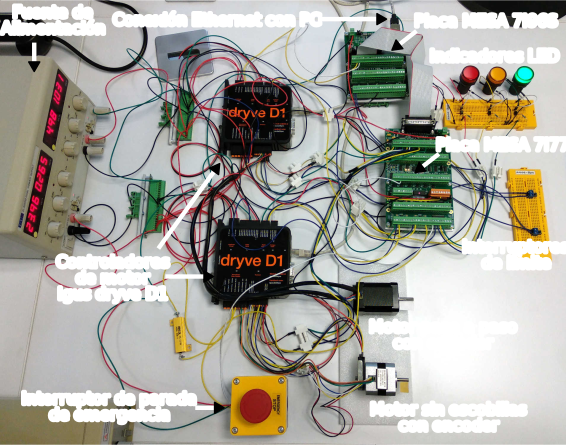
\includegraphics[width=1\linewidth]{images/installation/installation_labelled.pdf}
    \caption{Montaje de prueba.}
    \label{fig:installation}
\end{figure}


\begin{itemize}
    \item \textbf{Fuente de alimentación doble Aim-TTI EL302RD}: Proporciona dos fuentes de alimentación con un máximo de \qty{30}{\V} y \qty{2}{\A} cada una. En el montaje de prueba hemos necesitado alimentación de \qty{24}{\V} y \qty{5}{\V}.
    
    \item \textbf{2 controladores de motores \href{https://www.igus.eu/product/D1}{Igus dryve D1}}: Los controladores Igus dryve D1 son dispositivos utilizados para controlar motores paso a paso, de corriente continua, y sin escobillas en aplicaciones industriales y de automatización.
    Los Igus dryve D1 admiten las siguientes formas de interacción con sistemas de control:
    \begin{itemize}
        \item \textbf{CANopen}: Protocolo de comunicación usado en sistemas de automatización industrial, basado en el bus CAN (ISO 11898).
            
        \item \textbf{Modbus TCP}: Protocolo de comunicación ampliamente utilizado en aplicaciones industriales para la transmisión de datos en redes Ethernet sobre el protocolo TCP.
    
        \item \textbf{Señales analógicas y digitales}: Además de las opciones de comunicación en red, los dryve D1 pueden recibir señales analógicas y digitales para el control directo.
    \end{itemize}

    En nuestro caso nos comunicamos con los controladores Igus dryve D1 mediante las placas MESA 7I96S y 7I77 usando señales digitales y analógicas. De esta forma, podemos emplear LinuxCNC para tener un control preciso y en tiempo real sobre el funcionamiento de los motores en el sistema.

    
    \item \textbf{Placa \href{http://store.mesanet.com/index.php?route=product/product&product_id=374}{MESA 7I96S}}: Es la interfaz de hardware principal entre LinuxCNC y los controladores Igus dryve D1. Esta placa está conectada a la computadora que ejecuta LinuxCNC a través de una conexión Ethernet. Sus funciones principales incluyen:
    \begin{itemize}
        \item Controlar el motor paso a paso enviando señales de paso y dirección al controlador Igus dryve D1 correspondiente.
        
        \item Recibir las señales de los interruptores de límite.
    \end{itemize}
    
    \item \textbf{Placa hija \href{http://store.mesanet.com/index.php?route=product/product&product_id=120}{MESA 7I77}}: Está conectada a la placa 7i96S mediante un cable plano de 25 pines. Sus funciones principales incluyen:
    \begin{itemize}
        \item Controlar el motor sin escobillas enviando una señal analógica de velocidad al controlador Igus dryve D1 correspondiente.
        
        \item Recibir las señales de posición de los encoders de los motores.
        
        \item Recibir las señales de advertencia y error provenientes de los controladores.

        \item Recibir la señal de parada de emergencia al presionar el interruptor de parada de emergencia.
    \end{itemize}

    \item \textbf{Motor sin escobillas}: \href{https://www.omc-stepperonline.com/24v-4000rpm-0-0625nm-26w-1-8a-42x42x40mm-brushless-dc-motor-42bls40-24-01}{STEPPERONLINE 42BLS40-24-01}, con un codificador óptico \href{https://www.cuidevices.com/product/motion-and-control/rotary-encoders/incremental/modular/amt10-series}{CUI Devices AMT102-0512-I5000-S} de 512 \ac{PPR}.
    
    \item \textbf{Motor paso a paso}: \href{https://www.omc-stepperonline.com/nema-17-closed-loop-stepper-motor-65ncm-92oz-in-with-magnetic-encoder-1000ppr-4000cpr-17hs24-2104-me1k}{STEPPERONLINE 17HS24-2104-ME1K}. Incluye codificador magnético de 1000 \ac{PPR}.
    
    \item \textbf{Indicadores LED}: Sistema de desarrollo propio con LEDs rojo, amarillo y verde, que permite mostrar visualmente el estado del sistema.
    
    \item \textbf{2 botones para simular sensores de límites}.
        
    \item \textbf{Interruptor de parada de emergencia}: Dispone de un contacto normalmente cerrado y un contacto normalmente abierto.
\end{itemize}

El esquema de conexionado del sistema, donde se especifican todos los componentes usados y sus conexiones, se proporciona en el archivo \texttt{pruebas\_robot.pdf}.


\section{Controladores Igus dryve D1}

En esta sección, describiremos en detalle la configuración de los controladores Igus dryve D1. Para configurar los controladores es necesario conectarlos mediante Ethernet a un PC. Si no sabemos la dirección IP de un controlador podemos obtenerla al encenderlo o reconectar el cable Ethernet, en estos casos el controlador mostrará su dirección IP dígito a dígito en el visualizador de siete segmentos de su frontal.

\begin{figure}[!ht]
    \centering
    \includegraphics[width=1\linewidth,clip=true,trim=0 50px 650px 0]{images/config-stepper/01-start.png}
    \caption{Página de configuración inicial del controlador del motor paso a paso.}
    \label{fig:conf_stepper_1}
\end{figure}

Una vez conectados los controladores, abriremos un navegador web y pondremos la dirección IP del controlador que queramos configurar, esto nos permitirá acceder a la interfaz web de configuración del controlador. En la \cref{fig:conf_stepper_1} se muestra la página principal de configuración del controlador del motor paso a paso.

En las siguientes secciones se describen los parámetros de configuración del controlador y los valores a aplicar en cada parámetro para el motor sin escobillas y el motor paso a paso. Para una información más detallada se recomienda consultar el manual de los controladores (ver archivo «\texttt{Operating Manual dryve D1 EN V3.0.1.pdf}»).

\subsection{Página «Start»}
\label{sec:conf_start}

La página de configuración «Start» se muestra en la \cref{fig:conf_stepper_1}. Esta página contiene diversos ajustes generales. En particular, estableceremos las siguientes opciones en todos los controladores:

\begin{itemize}
    \item \textbf{Measuring system}: Metric, Millimeter
    \item \textbf{Movement type}: Rotary
    \item \textbf{Time units}: Seconds
\end{itemize}


\begin{admonition}{Nota}
    Hemos configurado la opción de tipo de movimiento (\textit{Movement type}) como rotatorio (\textit{Rotary}) aunque el motor mueva un eje lineal. Esto es porque en nuestro caso no necesitamos que el controlador controle la posición del eje, ya que de esto se encargará LinuxCNC, solo necesitamos que responda a las señales de movimiento que le mandemos. Esto además puede facilitar la configuración de los parámetros de movimiento del motor en las páginas «Axis» (ver \cref{sec:page_axis}) y «Drive Profile» (ver \cref{sec:page_drive_profile}).
\end{admonition}

Además, esta página también tiene las siguientes secciones:

\begin{itemize}
    \item \textbf{Configuration}: Permite guardar la configuración actual del controlador a archivo y cargar una configuración desde archivo. Una vez se haya terminado de definir la configuración del controlador se recomienda usar esta funcionalidad para guardarla en un archivo. 
    
    \item \textbf{Firmware}: Permite actualizar el firmware del controlador. El botón «Search» dirige a la URL de descarga de la última versión del firmware. El botón «Update» permite cargar el archivo de firmware desde disco para actualizar el controlador.
    
    \item \textbf{Password}: Permite establecer contraseña para los usuarios «Admin» (administrador) y «Guest» (invitado). Los usuarios pueden activarse o desactivarse con los interruptores correspondientes. Si ambos usuarios están desactivados (valor por defecto), se accede a la interfaz de usuario como «Admin». El usuario «Guest» sólo puede activarse si previamente se ha activado el usuario «Admin».
\end{itemize}


\subsection{Página «Motor»}

La página de configuración «Motor» se muestra en la \cref{fig:conf_stepper_2}. A continuación se describen las distintas opciones disponibles en esta página y como deben ser establecidas.


\begin{figure}[!ht]
    \centering
    \includegraphics[width=1\linewidth,clip=true,trim=0 25px 650px 0]{images/config-stepper/02-motor.png}
    \caption{Página de configuración de «motor» del controlador del motor paso a paso.}
    \label{fig:conf_stepper_2}
\end{figure}


\subsubsection{Motor}
\label{sec:motor_motor}

\begin{itemize}
    \item \textbf{Motor Type}: El tipo de motor, en nuestro caso seleccionamos «EC/BLDC (Brush-Less DC Motor)» para el motor sin escobillas, o «ST (Stepper Motor)» para el motor paso a paso.

    \item \textbf{Article Number}: Para motores Igus podemos seleccionar el número de articulo del motor. En este caso los parámetros «Motor Current», «Boost Current», «Holding Current», «Step Angle», y «Pole pairs», así como los demás parámetros de las secciones «Gear», «Feedback», «Closed Loop», «Brake», y «Braking Resistor», se rellenan automáticamente con los valores por defecto correspondientes al modelo de motor seleccionado.
    
    En el montaje de prueba, como estamos usando otros motores, hemos seleccionado «Custom article».

    \item \textbf{Motor Current (A)}: Indica la corriente continua máxima permisible del motor durante movimientos continuos, i.e., excepto en las fases de aceleración y desaceleración (ver la opción «Boost Current» para estos casos). Los valores posibles son de \qtyrange{0}{7}{\A}.

    \begin{admonition}{Importante}
        Este parámetro debe ser menor que la corriente máxima que pueda proporcionar la fuente de alimentación, teniendo también en cuenta las demás posibles cargas a las que deba suministrar potencia la fuente.
    \end{admonition}

    En el montaje de prueba, como ambos motores son pequeños, no tienen ninguna carga que mover, y la fuente de alimentación usada proporciona un máximo de 2A, hemos establecido valores pequeños en este parámetro: \qty{0.3}{\A} para el motor paso a paso y \qty{1}{\A} para el motor sin escobillas.

    \item \textbf{Boost Current (A)}: Corriente de refuerzo. Indica la corriente máxima permisible del motor durante las fases de aceleración y deceleración. Durante estas fases, es posible un aumento de la corriente motor establecida en el parámetro «Motor Current» hasta el valor de la corriente de refuerzo durante un máximo de \qty{2}{\s}. La activación de la corriente de refuerzo depende de la frecuencia de movimiento. Los valores posibles son desde el valor del parámetro «Motor Current» hasta el \qty{150}{\percent} (para motores paso a paso) o el \qty{300}{\percent} (para motores sin escobillas) del valor del parámetro «Motor Current».

    \begin{admonition}{Importante}
        Al igual que en el parámetro anterior, este parámetro debe ser menor que la corriente máxima que pueda proporcionar la fuente de alimentación, teniendo también en cuenta las demás posibles cargas a las que deba suministrar potencia la fuente.
    \end{admonition}

    En el montaje de prueba, al igual que en el parámetro anterior, hemos establecido valores pequeños en este parámetro: 0.5 A para el motor paso a paso y 1 A para el motor sin escobillas.
    
    \item \textbf{Holding Current (A)}: Corriente de retención. Ajusta la corriente aplicada al motor si está parado. Solo aplicable al caso de motores paso a paso en circuito de bucle abierto, en otro caso el parámetro estará deshabilitado y aparecerá sombreado en gris.

    En el montaje de prueba hemos configurado el controlador en bucle cerrado, por lo que esta opción está deshabilitada.
    
    \item \textbf{Step Mode}: Modo de paso. Solo aplicable en motores paso a paso, en otro caso el parámetro estará deshabilitado y aparecerá sombreado en gris. Este parámetro permite configurar la técnica de «microstepping» para controlar el motor \cite{electricmotorsanddrives,enwiki:1166298756}. En lugar de mover el motor un paso completo a la vez (modo de paso 1/1), la técnica de microstepping divide cada paso en fracciones más pequeñas, lo que permite un mayor número de posiciones intermedias. Los modos disponibles son «Auto», 1/1 (paso completo), 1/2, 1/4, 1/8, 1/16, 1/32, y 1/64.
    
    Cuanto menor sea el paso, más preciso será el posicionamiento, mejor será la estabilidad del movimiento, y menos ruido se emitirá, pero por otra parte la velocidad máxima teórica disminuirá. Por ejemplo, para un motor con un ángulo de paso de \ang{1.8}, en modo de paso 1/1 se necesitan 200 pasos para completar un giro. En general, para un ángulo de paso $\theta$ y modo de paso $1/N$ se necesitan $360N/\theta$ pasos para completar un giro. Considerando que el controlador puede procesar pulsos de paso con un período de pulso mínimo $T$, la velocidad máxima teórica del motor en rpm será de $60\theta/(360NT) = \theta/(6NT)$. Es decir, para un modo de paso $1/N$, la velocidad máxima teórica se verá reducida por un factor $N$ con respecto a la velocidad máxima teórica del modo 1/1.
    
    La documentación del Igus dryve D1 especifica un período mínimo de pulso de paso de \qty{40}{\us}. Sin embargo, el período mínimo real es menor. Utilizando un generador de señales y un osciloscopio hemos comprobado que el período mínimo real de pulso admitido por el Igus dryve D1 es de \qty{4}{\us}. En la \cref{tab:step_modes} se muestran para cada modo de paso los pasos por revolución y las máximas velocidades teóricas en rpm considerando un ángulo de paso de \ang{1.8} y un período de pulso de paso mínimo de \qty{4}{\us}. Es importante destacar que las velocidades mostradas en la tabla son velocidades teóricas calculadas a partir de la formula $\theta/(6NT)$, en la práctica los motores paso a paso no están pensados para llegar a altas velocidades. La máxima velocidad de un motor paso a paso dependerá del modelo de motor, pero normalmente la velocidad máxima de estos motores no será superior a \qty{1000}{rpm}.

    En el montaje de prueba hemos establecido el modo de paso 1/32.


    \begin{table}[!ht]
        \centering
        \begin{tabular}{
            c
            S[table-format=5]
            S[table-format=5]
        }
            \toprule
            Modo de paso &
            \multicolumn{1}{c}{Pasos por revolución} &
            \multicolumn{1}{c}{Máxima velocidad (rpm)} \\
            \midrule
             1/1 &   200 & 75000 \\
             1/2 &   400 & 37500 \\
             1/4 &   800 & 18750 \\
             1/8 &  1600 &  9370 \\
            1/16 &  3200 &  4680 \\ 
            1/32 &  6400 &  2340 \\
            1/64 & 12800 &  1170 \\
            \bottomrule
        \end{tabular}
        \caption{Modos de paso, pasos por revolución, y máximas velocidades teóricas en rpm considerando un ángulo de paso de \ang{1.8} y un período de pulso de paso mínimo de \qty{4}{\us}.}
        \label{tab:step_modes}
    \end{table}


    \item \textbf{Step Angle}: Ángulo de paso. Solo disponible para motores paso a paso. El ángulo de paso indica el ángulo de un paso completo del motor (e.g., \ang{0.72}, \ang{0.9}, \ang{1.8}). Esto es un parámetro físico del propio motor y determina el número de pasos completos por revolución, e.g., un motor con un ángulo de paso de \ang{1.8} necesita $360/1.8 = 200$ pasos completos por revolución.

    En el montaje de prueba el motor paso a paso usado tiene un ángulo de paso de \ang{1.8}.

    \item \textbf{Pole Pairs}: Pares de polos. Solo disponible para motores sin escobillas. Indica el número y la disposición de las bobinas del motor. Es un parámetro físico del propio motor.

    En el montaje de prueba el motor sin escobillas usado tiene 4 pares de polos.
\end{itemize}


Una vez rellenados los campos de esta sección deberemos hacer clic en el botón «Apply Changes».


\subsubsection{Gear}

Si el motor dispone de un engranaje reductor, este se puede configurar en esta sección. Estableceremos esta opción a «OFF».

\begin{admonition}{Nota}
    Estableceríamos esta opción a «OFF» aunque el motor dispusiera de engranaje reductor. Esta opción solo sería necesaria si quisiéramos que el controlador controlara la posición de su eje, pero como se comentó en \cref{sec:conf_start}, en nuestro caso no lo necesitamos, ya que de esto se encargará LinuxCNC, solo necesitamos que el controlador responda a las señales de movimiento que le mandemos. Esto además puede facilitar la configuración de los parámetros de movimiento del motor en las páginas «Axis» (ver \cref{sec:page_axis}) y «Drive Profile» (ver \cref{sec:page_drive_profile}).
\end{admonition}

\subsubsection{Feedback}

Esta sección permite configurar los parámetros del encoder conectado al controlador. Si en el parámetro «Article Number» de la sección «Motor» hemos seleccionado un motor de Igus, los parámetros de esta sección ya estarán establecidos a sus valores correctos.

En el montaje de prueba hemos establecido los siguientes valores, de acuerdo con las especificaciones de los encoders correspondientes:

\begin{itemize}
    \item \textbf{Motor paso a paso}
    \begin{itemize}
        \item \textbf{Tipo}: Encoder as a Line Driver
        \item \textbf{Index}: ON
        \item \textbf{Impulses}: 1000
    \end{itemize}
    
    \item \textbf{Motor sin escobillas}
    \begin{itemize}
        \item \textbf{Tipo}: Encoder as Single Ended
        \item \textbf{Index}: ON
        \item \textbf{Impulses}: 512
    \end{itemize}
\end{itemize}

\begin{admonition}{Importante}
    El botón «Impulse Check» hace al controlador comprobar automáticamente el número de impulsos del encoder. Para esto hace girar una revolución el motor, incluso aunque la señal «enable» no esté activada. Por lo tanto, es importante no hacer clic en este botón si el motor no puede girar libremente.
\end{admonition}


\subsubsection{Closed Loop}

Mediante el control de bucle cerrado el controlador compara la información de posición recibida del encoder con el valor de referencia deseado y ajusta el motor en función de esa comparación. Esta retroalimentación continua permite corregir errores, manteniendo el motor en la posición, velocidad, o estado deseado, y adaptarse a las variaciones de carga de manera más eficiente, lo que resulta en un control preciso y estable del motor, reduciendo considerablemente su consumo de energía y su temperatura de funcionamiento.

Establecemos esta opción a «ON».

\begin{admonition}{Importante}
    Para el control de bucle cerrado, el Igus dryve D1 utiliza internamente dos controladores \acp{PI} para controlar la corriente y la velocidad, respectivamente, y un controlador \ac{P} para controlar la posición. Los parámetros de estos controladores se muestran en la página «Oscilloscope» (ver \cref{sec:oscilloscope_parameters}). Si se pulsa en el botón «Self Tuning» de esta sección, el controlador intentará determinar automáticamente los valores de los parámetros de estos controladores.
\end{admonition}


\subsubsection{Brake}

El Igus dryve D1 puede controlar un freno de retención. Ninguno de los motores que tenemos dispone de freno así que establecemos esta opción a «OFF».


\subsubsection{Braking Resistor}

Esta sección solo es aplicable al caso de motores sin escobillas. Estos motores, al desacelerar, funcionan como generadores de potencia. Esto puede producir picos de tensión mayores que la tensión de carga aplicada, lo cual puede causar la destrucción del controlador, sobre todo en el caso de altas desaceleraciones. Para evitar daños al controlador, se debe utilizar una resistencia de frenado para disipar la energía excesiva generada. Por lo tanto, es importante que cada controlador que accione un motor sin escobillas esté equipado con su propia resistencia de frenado.

El valor de la resistencia y su capacidad de disipación de potencia dependen del motor usado. El manual del controlador proporciona los detalles de como obtener estos valores a partir de los datos del motor. En el montaje de prueba hemos usado una resistencia de \qty{33}{\ohm} con una potencia de disipación máxima a \qty{25}{\degreeCelsius} de \qty{50}{\W} (con disipador estándar) o \qty{14}{\W} (sin disipador).

Esta sección proporciona un único parámetro «Braking Voltage (V)», que establece el umbral de tensión para aplicar la resistencia de frenado y disipar el exceso de energía. Para una operación segura, el controlador considera una histéresis de \qty{1}{\V}, de forma que la resistencia de frenado se activará cuando la tensión del motor llegue a la tensión umbral más \qty{1}{\V}, y se detendrá cuando baje hasta la tensión umbral menos \qty{1}{\V}.

El umbral de tensión establecido en el parámetro «Braking Voltage» debe ser un valor ligeramente superior a la tensión de alimentación del motor, por ejemplo, si la tensión de alimentación del motor es \qty{24}{\V} un umbral adecuado puede ser \qty{26}{\V}, si la tensión de alimentación del motor es \qty{48}{\V}, un umbral adecuado puede ser \qty{51}{\V}. Un valor demasiado alto podría causar que se disipase poca energía y causar el error «E09 Load Supply High» (ver el manual del controlador, Sección 7: Alerts and Errors).

En el montaje de prueba el motor sin escobillas usado estaba alimentado a \qty{24}{\V}, así que hemos establecido este parámetro a \qty{26}{\V}.


\subsection{Página «Axis»}
\label{sec:page_axis}

La página de configuración «Axis» se muestra en la \cref{fig:conf_stepper_3}. Como se puede ver en la figura, los parámetros usan las unidades establecidas en la página de configuración inicial (ver \cref{sec:conf_start}), así, los de posición están en grados (\unit{\degree}), los de velocidad en grados por segundo (\unit{\degree/\s}), y los de aceleración en grados por segundo al cuadrado (\unit{\degree/\s^2}). A continuación se describen las distintas opciones disponibles en esta página y como deben ser establecidas.

\begin{figure}[!ht]
    \centering
    \includegraphics[width=1\linewidth,clip=true,trim=0 25px 650px 0]{images/config-stepper/03-axis.png}
    \caption{Página de configuración de «eje» del controlador del motor paso a paso.}
    \label{fig:conf_stepper_3}
\end{figure}


\subsubsection{Axis}

Esta sección contiene los siguientes parámetros:

\begin{itemize}
    \item \textbf{Available Stroke}: Establece la ventana de movimiento para el modo «ABS» (Absolute Positioning). No usaremos este modo, así que este parámetro es irrelevante para nosotros.

    \item \textbf{Feed Rate}: En ejes lineales este parámetro indica el desplazamiento del eje por rotación del motor. Nosotros consideramos un eje rotatorio y en este caso debemos establecer este parámetro a \ang{360} tal y como indica el manual del controlador en su Sección 5.5.1.
\end{itemize}


\subsubsection{Motion Limits}
\label{sec:axis_motion_limits}

Esta sección contiene los siguientes parámetros:

\begin{itemize}
    \item \textbf{Max. Velocity (\unit{\degree/\s})}: Máxima velocidad del motor. Sirve como límite en los modos de programación de movimientos disponibles en la página «Drive Profile» (ver \cref{sec:page_drive_profile}). En el caso del motor paso a paso la velocidad estará controlará mediante la señal de paso que recibirá el controlador, por lo que queremos que este parámetro sea lo mayor posible. En el caso del motor sin escobillas la velocidad máxima se establecerá en la página «Drive Profile», con un valor no superior al establecido en este parámetro. Por lo tanto estableceremos este parámetro a su valor máximo: \qty{100000}{\degree/\s}.

    \item \textbf{Jog Velocity (\unit{\degree/\s})}: Velocidad del motor para el posicionamiento manual disponibles en la página «Drive Profile» (ver \cref{sec:page_drive_profile}). Este parámetro solo es útil para realizar pruebas desde la interfaz web del controlador, en nuestro caso lo hemos establecido a \qty{360}{\degree/\s}. Para el sistema final este parámetro es irrelevante.

    \item \textbf{Max. Acceleration (\unit{\degree/\s^2})}: Aceleración máxima del motor. Es la aceleración usada en el posicionamiento manual disponible en la página «Drive Profile» (ver \cref{sec:page_drive_profile}). También sirve como límite en los modos de programación de movimientos disponibles en la página «Drive Profile». Al igual que la velocidad, para el caso del motor paso a paso la aceleración estará controlará mediante la señal de paso que recibirá el controlador. En el caso del motor sin escobillas la aceleración máxima también se establecerá en la página «Drive Profile», con un valor no superior al establecido en este parámetro. Por lo tanto estableceremos este parámetro a su valor máximo: \qty{1000000}{\degree/\s^2}.

    \item \textbf{S-Curve (\unit{\percent})}: Permite controlar la tasa de cambio de la aceleración, conocida como «jerk» \cite{enwiki:1178778094}. Puede ajustarse entre \qty{0}{\percent} y \qty{100}{\percent} para controlar la suavidad de las transiciones de aceleración y desaceleración en el movimiento del motor.
    %
    Valores más bajos producirán cambios bruscos en la aceleración, lo que genera niveles de «jerk» más altos y, en consecuencia, movimientos menos suaves que pueden causar vibraciones no deseadas y tensiones en el sistema. En contraste,  valores más altos reducirán el «jerk», lo que resulta en transiciones de aceleración y desaceleración más suaves, minimizando las vibraciones y el desgaste en el motor y la maquinaria.

    Si deseamos que un controlador externo (como LinuxCNC) tenga un control total sobre el movimiento del motor estableceremos este parámetro a \qty{0}{\percent}. En este caso, se desactiva cualquier suavizado de transiciones de aceleración y desaceleración dentro del propio controlador del motor, permitiendo que el controlador externo gestione directamente el movimiento.

    Sin embargo, el controlador de movimiento actual de LinuxCNC no dispone de limitación del «jerk», i.e., usa aceleración constante. Podría ser deseable establecer en este parámetro un valor mayor que \qty{0}{\percent} para limitar el «jerk» y evitar vibraciones no deseadas y tensiones en el sistema. Sin embargo, esto tendría la desventaja de aumentar el error de seguimiento dentro de LinuxCNC. Por lo tanto, en caso de querer establecer esta opción a un valor mayor que \qty{0}{\percent} sería importante encontrar un equilibrio entre la suavidad del movimiento y la precisión del seguimiento.

    En nuestro caso hemos establecido el parámetro a \qty{0}{\percent}.
    
    \item \textbf{Quick-Stop (\unit{\degree/\s^2})}: Desaceleración cuando se detiene un movimiento en caso de emergencia. Se ejecutará una parada rápida en el caso de que se revoque la señal de «Enable» (entrada digital X2.7) del controlador.

    \begin{admonition}{Importante}
        Es necesario asegurarse de que la desaceleración especificada sea adecuada para la aplicación prevista. Una desaceleración demasiado baja podría tardar demasiado tiempo en detener el movimiento del robot, por otra parte una desaceleración demasiado elevada podría dañar la estructura mecánica del robot.
    \end{admonition}

    En el montaje de prueba hemos establecido este parámetro a \qty{50000}{\degree/\s^2}.

    \item \textbf{Following Error (\unit{\degree})}: Desviación admisible de la posición real con respecto a la posición deseada. Si se alcanza el \qty{50}{\percent} del error de seguimiento permitido, se emite un aviso (warning). Si se supera el error de seguimiento permitido, el movimiento se detiene y se emite un error.

    En el montaje de prueba hemos establecido este parámetro a \ang{20}.
    
    \item \textbf{Positioning Window (\unit{\degree})}: Ventana de posicionamiento. Se utiliza para definir un rango de posición alrededor de un punto de destino en una dirección positiva y negativa. Por ejemplo, si el objetivo es llegar a \qty{100}{\mm} y se establece una ventana de posicionamiento de \qty{10}{\mm}, el sistema considerará que la posición está dentro del rango objetivo si se encuentra en cualquier lugar entre \qty{90}{\mm} y \qty{110}{\mm}. Si la posición real del motor se encuentra dentro de esta ventana, se considera que el movimiento ha finalizado, incluso si el motor está bloqueado mecánicamente. Esto se hace para evitar que el sistema continúe intentando alcanzar una posición exacta en caso de bloqueo. Si la ventana de posicionamiento se establece a 0, se desactiva esta función y el sistema no tomará en cuenta el rango alrededor del punto de destino.

    En el montaje de prueba hemos establecido este parámetro a 0, por lo tanto esta función está desactivada.

    \item \textbf{Positioning Time (\unit{\ms})}: Tiempo de posicionamiento. Especifica cuánto tiempo debe mantenerse la posición real dentro del rango definido por la ventana de posicionamiento antes de que se considere que un movimiento ha finalizado. Este tiempo se establece en milisegundos y sirve como una medida de estabilidad y precisión en el posicionamiento.

    En el montaje de prueba hemos establecido este parámetro a 0.
\end{itemize}


\subsubsection{Limit Switch}
\label{sec:limit_switch}
Incluye un parámetro «Position» que permite especificar la posición y el número de sensores de límites usados. 

En el montaje de prueba los sensores de límites no se conectan a los controladores, solo se conectan a la placa MESA 7I96S, de forma que los límites son gestionados íntegramente por LinuxCNC. Por lo tanto establecemos el parámetro «Position» a «None».


\subsubsection{Reference}

Permite seleccionar el método de referencia («homing») preferido y el  desplazamiento de posición («offset»).

Al igual que los límites de movimiento robot (ver \cref{sec:limit_switch}), el proceso de «homing» también estará controlado íntegramente por LinuxCNC. Por lo tanto hemos establecido los siguientes parámetros:

\begin{itemize}
    \item \textbf{Method}: SCP (Set Current Position)
    \item \textbf{Offset (\unit{\degree})}: 0
\end{itemize}


\subsubsection{Absolute Feedback}
\label{sec:axis_absolute_feedback}

El controlador Igus Drive D1 dispone de dos entradas analógicas, AI 1 (Analog Input 1, entrada X4.1) y AI 2 (Analog Input 2, entrada X4.2), que se utilizan para configurar y controlar la posición o velocidad objetivo y la posición actual del sistema, respectivamente. En nuestro sistema usaremos la entrada analógica AI 1 para controlar la velocidad del motor sin escobillas, la entrada analógica AI 2 no sé usará. En el caso del motor paso a paso no se usarán estas entradas, por lo tanto esta sección solo es relevante para el motor sin escobillas. A continuación se describen los para parámetros relativos a las entradas analógicas disponibles en esta sección.


\begin{itemize}
    \item \textbf{Parámetros relativos a AI 1 (entrada X4.1)}:
    
    La entrada AI 1 se usará para controlar la velocidad del motor sin escobillas (ver \cref{sec:page_drive_profile}). El voltaje de control analógico de entrada será de \qty{\pm10}{\V}, lo cual deberá configurarse en la página «Inputs/Outputs» (ver \cref{sec:page_input_outputs}), y habrá que tenerlo en cuenta a la hora de establecer los parámetros relativos a AI 1 que se indican a continuación.
    
    \begin{itemize}
        \item \textbf{AI 1 Target Value Min. (\unit{\V})}: Valor de tensión mínimo en la entrada analógica AI 1. Establecemos su valor a \qty{-10}{\V}.
  
        \item \textbf{AI 1 Target Value Max. (\unit{\V})}: Valor de tensión máximo en la entrada analógica AI 1. Establecemos su valor a \qty{10}{\V}.
  
        \item \textbf{AI 1 Dead Band Zero Value (\unit{\V})}: Permite establecer una banda muerta colocada simétricamente alrededor de \qty{0}{V} en la señal objetivo correspondiente a la entrada analógica AI 1. Este parámetro se puede especificar en pasos de \qty{0.001}{\V}. Establecemos su valor a \qty{0}{\V}.
  
        \item \textbf{AI 1 Dead Band Input Signal (\unit{\V})}: Permite establecer una banda muerta colocada simétricamente alrededor de \qty{0}{V} en la señal de entrada de la Entrada Analógica AI 1. Este parámetro se puede especificar en pasos de \qty{0.001}{\V}. Establecemos su valor a \qty{0}{\V}.
  
        \item \textbf{AI 1 Filter (\unit{\ms})}: Intervalo para promediar la señal. Se utiliza para filtrar las variaciones bruscas de la señal y evitar inconsistencias en el movimiento. Valores bajos resultan en un sistema que responde rápidamente pero que es más susceptible al ruido o interferencias. Valores altos resultan en un sistema más estable pero con un mayor tiempo de respuesta. Establecemos su valor a \qty{10}{\ms}.
    \end{itemize}


    Los parámetros de banda muerta, «AI 1 Dead Band Zero Value» y «AI 1 Dead Band Input Signal», se pueden usar para minimizar movimientos no deseados del motor durante el estado de reposo causados por un mayor rizado de la señal de entrada u otras interferencias. Considerando los anteriores parámetros, si tenemos el voltaje analógico de entrada $x$ ya filtrado según lo especificado en el parámetro «AI 1 Filter», la posición o velocidad objetivo se calculará mediante las siguientes funciones de transferencia:
    
    \begin{itemize}
        \item $f_{\text{ZV}}(\cdot)$, correspondiente al parámetro «AI 1 Dead Band Zero Value» y mostrada en la \cref{fig:deadband_zv}.
        \item $f_{\text{IS}}(\cdot)$, correspondiente al parámetro «AI 1 Dead Band Input Signal» y mostrada en la \cref{fig:deadband_is}.
    \end{itemize}
    
    de forma que para el valor analógico de entrada $x$ la posición o velocidad objetivo será:
    
    \begin{equation}
        y = (f_{\text{ZV}} \circ f_{\text{IS}})(x) = f_{\text{ZV}}(f_{\text{IS}}(x))
    \end{equation}

    \begin{admonition}{Nota}
        El cálculo de la posición o velocidad objetivo no está especificado en el manual del controlador (considerando la versión del manual 3.0.1, la más reciente a fecha de este documento) y se ha obtenido experimentalmente. El manual solo describe los parámetros «AI 1 Dead Band Zero Value» y «AI 1 Dead Band Input Signal» de manera textual, de forma similar a como se han descrito más arriba.
    \end{admonition}

    \begin{figure}[!ht]
        \centering
        \begin{tikzpicture}
    \def\VMax{10}
    \def\VDeadBand{3}
    
    \begin{axis}[
        % height=6cm,
        % width=10cm,
        xlabel={Input voltage (\unit{\V})},
        ylabel={Target position or velocity},
        xmin=-11,
        xmax=11,
        ymin=-1.25,
        ymax=1.25,
        xtick={-\VMax, -\VDeadBand, 0, \VDeadBand, \VMax},
        xticklabels={
            $-V_{\text{max}}$,
            $-V_{\text{ZVdb}}$,
            0,
            $V_{\text{ZVdb}}$,
            $V_{\text{max}}$
        },
        ytick={-1, 0, 1},
        yticklabels={$-o_{\text{max}}$, 0, $o_{\text{max}}$},
        grid=both,
    ]
    % Recta 1
    \addplot [domain=-\VMax:-\VDeadBand, thick] {(x + \VDeadBand)/(\VMax - \VDeadBand)};

    % Recta 2
    \addplot [domain=-\VDeadBand:\VDeadBand, thick] {0};

    % Recta 3
    \addplot [domain=\VDeadBand:\VMax, thick] {(x - \VDeadBand)/(\VMax - \VDeadBand)};
    
    \end{axis}
\end{tikzpicture}
        \caption{Función de transferencia $f_{\text{ZV}}(\cdot)$.}
        \label{fig:deadband_zv}
    \end{figure}
    
    \begin{figure}[!ht]
        \centering
        \begin{tikzpicture}
    \def\VMax{10}
    \def\VDeadBand{3}
    
    \begin{axis}[
        % height=6cm,
        % width=10cm,
        xlabel={Input voltage (\unit{\V})},
        ylabel={Output voltage (\unit{\V})},
        xmin=-11,
        xmax=11,
        ymin=-11,
        ymax=11,
        xtick={-\VMax, -\VDeadBand, 0, \VDeadBand, \VMax},
        xticklabels={
            $-V_{\text{max}}$,
            $-V_{\text{ISdb}}$,
            0,
            $V_{\text{ISdb}}$,
            $V_{\text{max}}$
        },
        ytick={-\VMax, -\VDeadBand, 0, \VDeadBand, \VMax},
        yticklabels={
            $-V_{\text{max}}$,
            $-V_{\text{ISdb}}$,
            0,
            $V_{\text{ISdb}}$,
            $V_{\text{max}}$
        },
        grid=both,
    ]
    % Recta 1
    \addplot [domain=-\VMax:-\VDeadBand, thick] {x};

    % Recta 2
    \addplot [thick,dashed] coordinates {(-\VDeadBand,-\VDeadBand) (-\VDeadBand,0)};
    \addplot [domain=-\VDeadBand:\VDeadBand, thick] {0};
    \addplot [thick,dashed] coordinates {(\VDeadBand,0) (\VDeadBand,\VDeadBand)};

    % Recta 3
    \addplot [domain=\VDeadBand:\VMax, thick] {x};
    
    \end{axis}
\end{tikzpicture}
        \caption{Función de transferencia $f_{\text{IS}}(\cdot)$.}
        \label{fig:deadband_is}
    \end{figure}


    \item \textbf{Parámetros relativos a AI 2 (entrada X4.2)}:\hfill

    La entrada analógica AI 2 sirve para proporcionar información de posición al controlador mediante una señal analógica. En nuestro caso no usaremos esta entrada, por lo que los parámetros relativos esta entrada son irrelevantes para nosotros.
    
    \begin{itemize}
        \item \textbf{AI 2 Absolute Value Min (\unit{\V})}: Valor de tensión mínimo en la entrada analógica AI 2.
  
        \item \textbf{AI 2 Absolute Value Max (\unit{\V})}: Valor de tensión mínimo en la entrada analógica AI 2.
    \end{itemize}
\end{itemize}


\subsection{Página «Communication»}
\label{sec:page_communication}

La página de configuración «Communication» se muestra en la \cref{fig:conf_stepper_4}. Esta página permite configurar las comunicaciones mediante Ethernet y los sistemas bus del controlador. A continuación se describen las distintas opciones disponibles en esta página y como deben ser establecidas.

\begin{figure}[!ht]
    \centering
    \includegraphics[width=1\linewidth,clip=true,trim=0 25px 650px 0]{images/config-stepper/04-communication.png}
    \caption{Página de configuración de «comunicación» del controlador del motor paso a paso.}
    \label{fig:conf_stepper_4}
\end{figure}


\subsubsection{Ethernet TCP/IP}

Esta sección permite configurar los parámetros de conexión TCP/IP: dirección IP, mascara de subred, puerta de acceso, y nombre del host. Una vez establecidos los parámetros se debe pulsar el botón «Reload» para aplicar los cambios.

En el montaje de prueba se han establecido estos parámetros de forma manual a los valores mostrados en la \cref{tab:conf_ethernet}. Los controladores se han conectado mediante un conmutador (switch) con un PC portátil. Los parámetros se establecieron para que fuera posible conectar el sistema a la red del laboratorio, aunque esto no se llegó a hacer.

\begin{table}[!ht]
    \centering
    \begin{tabular}{lll}
        \toprule
        Parámetro &  Motor paso a paso & Motor sin escobillas \\
        \midrule
        IP-Address & 10.68.33.120 & 10.68.33.121 \\
        Subnet Mask & 255.255.252.0 & 255.255.252.0 \\ 
        Gateway & 10.68.32.1 & 10.68.32.1 \\
        Hostname & igus-dryve-D1-098a & igus-dryve-D1-098e \\
        \bottomrule
    \end{tabular}
    \caption{Parámetros de configuración Ethernet.}
    \label{tab:conf_ethernet}
\end{table}


\subsubsection{Transmission Protocol}

Esta sección permite seleccionar si la comunicación con el servidor web del controlador dryve D1 debe hacerse mediante una conexión http no cifrada o una conexión https cifrada. En el caso de una conexión https se puede suministrar un certificado externo o generar un certificado autofirmado.

En el montaje de prueba se ha seleccionado la opción de usar una conexión http no cifrada.


\subsubsection{Bus Systems}

El controlador dispone de dos sistemas de buses, CANopen y Modbus, que permiten comunicarse con el controlador y controlar el movimiento del motor. En nuestro caso no usaremos ninguno de estos sistemas, ya que controlaremos el motor mediante las entradas y salidas de los conectores X2 (entradas digitales), X3 (salidas digitales), y X4 (entradas analógicas). Por lo tanto se han dejado las opciones «CANopen» y «Modbus TCP Gateway» al valor por defecto «OFF».


\subsection{Página «Inputs/Outputs»}
\label{sec:page_input_outputs}

La página de configuración «Inputs/Outputs» se muestra en la \cref{fig:conf_stepper_5}. Esta página permite configurar las entradas y salidas del controlador. 

\begin{figure}[!ht]
    \centering
    \includegraphics[width=1\linewidth,clip=true,trim=0 25px 650px 0]{images/config-stepper/05-inputs_outputs.png}
    \caption{Página de configuración de «Inputs/Outputs» del controlador del motor paso a paso.}
    \label{fig:conf_stepper_5}
\end{figure}

El nivel de la lógica digital usado por el controlador se establece alimentando la entrada X2.11 con un voltaje entre \qty{5}{\V} y \qty{24}{\V}. La lógica digital del controlador funciona de la siguiente forma:
\begin{itemize}
    \item Las salidas digitales se establecen a \qty{0}{\V} para nivel bajo (L) y al voltaje de X2.11 para nivel alto (H).

    \item Las entradas digitales se evaluarán a nivel bajo (L) para voltajes de \qtyrange{0}{10}{\percent} del voltaje de X2.11, y se evaluarán a nivel alto (H) para valores mayores que \qty{60}{\percent} del voltaje de X2.11.
\end{itemize}
Estos niveles se ilustran en la \cref{fig:controller_logic_levels}.

\begin{figure}[!ht]
    \centering
    \begin{tikzpicture}
    % Draw rectangle representing voltage levels
    \draw[fill=gray!20] (0,0) rectangle (3,6);
    
    % Mark voltage levels
    \draw[fill=white] (0,0.6) rectangle (3,3.6);

    \node[right] at (3,6) {Voltaje en X2.11};
    \node[right] at (3,3.6) {\qty{60}{\percent} de X2.11};
    \node[right] at (3,0.6) {\qty{10}{\percent} de X2.11};
    \node[right] at (3,0) {\qty{0}{\V}};

    % Add labels for logic states
    \node[] at (1.5, 4.8) {Valor alto};
    \node[] at (1.5, 2.1) {Valor indefinido};
    \node[] at (1.5, 0.3) {Valor bajo};

    % Draw arrows for voltage levels
    \draw[-{Stealth[length=3mm]}] (-1.5, 0) -- ++(0, 6.5) node[above,midway,rotate=90] {Voltaje};
\end{tikzpicture}

    \caption{Niveles de la lógica digital usada por el controlador.}
    \label{fig:controller_logic_levels}
\end{figure}

Para interactuar con las entradas y salidas digitales del controlador usamos las placas MESA 7I96S y 7I77:
\begin{itemize}
    \item La placa MESA 7I96S se usa para enviar las señales de paso y dirección al controlador del motor paso a paso, estas señales emplean lógica de \qty{5}{\V}.

    \item La placa MESA 7I77 se usa para enviar las señales «start» y «enable», y leer las salidas «ready», «alert», y «error» de los controladores (ver esquema de conexionado en el archivo \texttt{pruebas\_robot.pdf}). El voltaje de la lógica para la placa MESA 7I77 se puede ajustar alimentando la entrada TB2.1 («field power») con el voltaje deseado en un rango entre \qty{5}{\V} y \qty{28}{\V}.
\end{itemize}

Debido a que la placa MESA 7I96S solamente puede usar lógica de \qty{5}{\V} para las señales de paso y dirección, hemos establecido el voltaje de la lógica de los controladores Igus dryve D1 (entrada X2.11) y de la placa MESA 7I77 (entrada TB2.1) a \qty{5}{\V}. 

Las secciones disponibles en esta página son:

\begin{itemize}
    \item \textbf{Digital Inputs}: Muestra las entradas digitales y permite seleccionar para cada una entre normalmente abierta (H) o normalmente cerrada (L). Las entradas normalmente abiertas (H) se activarán cuando se reciba una señal alta. Por el contrario, las entradas normalmente cerradas se activarán cuando se reciba una señal baja (L). Dejaremos todas establecidas al valor por defecto (H).

    \begin{admonition}{Nota}
        Las etiquetas de las entradas digitales mostradas en esta página variarán dependiendo del modo de control del motor seleccionado en la página «Drive Profile» (ver \cref{sec:page_drive_profile}). En la \cref{fig:conf_stepper_5} se muestra la configuración del motor paso a paso, que muestra las entradas para el modo de control «step/direction».
    \end{admonition}

    \item \textbf{Digital Outputs}: Muestra las salidas digitales y permite seleccionar para cada una entre normalmente abierta (H) o normalmente cerrada (L). Dejaremos todas establecidas al valor por defecto (H).

    \item \textbf{Analog Inputs}: Muestra las entradas analógicas y permite establecer el rango de valores soportado de \qtyrange{0}{10}{\V} o de \qtyrange{-10}{10}{\V}. En nuestro caso usaremos la entrada analógica AI 1 con señales de \qtyrange{-10}{10}{\V} para controlar la velocidad del motor sin escobillas, como se comentó en la \cref{sec:axis_absolute_feedback}. Por lo tanto en el controlador del motor sin escobillas estableceremos la opción AI 1 al valor \qty{\pm10}{VDC}. La opción AI 2 la dejaremos sin modificar ya que no usaremos esa entrada.

    \item \textbf{Digital Input Switching}: Este parámetro determina cómo el sistema interpreta las señales de entrada digitales. Las opciones disponibles son PNP y NPN:
    \begin{itemize}
        \item \textbf{PNP} (sourcing): En el estado activado, la entrada se eleva al voltaje aplicado en X2.11. En el estado no activado, la entrada se lleva a tierra a través de una resistencia de «pull-down». En este caso, la corriente fluye desde la salida del sistema de control de nivel superior hasta la entrada del Igus dryve D1.
        
        \item \textbf{NPN} (sinking): En el estado activado, la entrada se lleva a tierra. En el estado no activado, la entrada se eleva al voltaje aplicado en X2.11 debido a una resistencia de «pull-up». En este caso, la corriente fluye desde la entrada del Igus dryve D1 hasta la salida del sistema de control de nivel superior.
    \end{itemize}

    En nuestro caso, todas las entradas y salidas de las placas MESA son de tipo PNP (sourcing), por lo que dejaremos establecida esta opción al valor por defecto «PNP».
\end{itemize}


\subsection{Página «Drive Profile»}
\label{sec:page_drive_profile}

Esta página permite seleccionar el modo de control para ejecutar movimientos.
Los modos disponibles son:

\begin{itemize}
    \item \textbf{Binary}: Control de movimiento mediante entradas digitales o analógicas y salidas digitales.
    
    \item \textbf{Tipp/Teach}: Control de movimiento mediante entradas digitales o analógicas y salidas digitales. En este modo es posible modificar las posiciones objetivo de movimientos existentes usando las entradas digitales.
    
    \item \textbf{Step/Direction}: Control de movimiento a partir de señales de paso y dirección. Solo disponible para motores paso a paso.
    
    \item \textbf{CANopen}: Control de movimiento a través del protocolo de comunicación CANopen.
    
    \item \textbf{Modbus TCP}: Control de movimiento a través del protocolo de comunicación Modbus TCP.
\end{itemize}

A continuación describimos las configuraciones a aplicar a los motores.


\subsubsection{Motor paso a paso}

En el caso del motor paso a paso seleccionamos el modo de control «step/direction». En la \cref{fig:conf_stepper_6} se muestra la página de configuración de «Drive Profile» del controlador del motor paso a paso, usando el modo de control «step/direction». Este modo de control no requiere de ninguna configuración adicional, en la página se mostrará la información de uso de las señales de paso y dirección.

\begin{figure}[!ht]
    \centering
    \includegraphics[width=1\linewidth,clip=true,trim=0 325px 575px 0]{images/config-stepper/06-drive_profile.png}
    \caption{Página de configuración de «Drive Profile» del controlador del motor paso a paso, usando el modo de control «step/direction».}
    \label{fig:conf_stepper_6}
\end{figure}


\subsubsection{Motor sin escobillas}

En el caso del motor sin escobillas seleccionamos el modo de control «binary». En la \cref{fig:conf_brushless_6} se muestra la página de configuración «Drive Profile» del controlador del motor sin escobillas, usando el modo de control «binary». Este modo proporciona una tabla de movimientos (ver la \cref{fig:conf_brushless_6}) que permite programar hasta 32 movimientos parametrizados con el modo de movimiento, el objetivo, la aceleración máxima, la velocidad, y el número del siguiente movimiento a ejecutar. Para el caso del motor sin escobillas introducimos un único movimiento en la posición 1 usando el modo ADR (Analogue Rotation with Direction Definition). El modo ADR permite realizar movimientos rotatorios estableciendo su velocidad en la entrada analógica AI 1.

\begin{figure}[!ht]
    \centering
    \includegraphics[width=1\linewidth,clip=true,trim=0 100px 250px 0]{images/config-brushless/06-drive_profile.png}
    \caption{Página de configuración de «Drive Profile» del controlador del motor sin escobillas, usando el modo de control «binary».}
    \label{fig:conf_brushless_6}
\end{figure}

En el montaje de prueba hemos establecido los siguientes parámetros para el movimiento de la posición 1:

\begin{itemize}
    \item \textbf{Mode}: ADR (Analogue Rotation with Direction Definition).
    \item \textbf{Goal (\unit{\degree})}: Lo dejaremos vacío.
    \item \textbf{Acceleration (\unit{\degree/\s^2})}: \qty{50000}{\degree/\s^2}, que equivalen a \qty{138.89}{rev/\s^2}.
    \item \textbf{Velocity (\unit{\degree/\s})}: \qty{18000}{\degree/\s}, que equivalen a \qty{3000}{rpm}.
    \item \textbf{Deceleration (\unit{\degree/\s^2})}: \qty{50000}{\degree/\s^2}, igual que la aceleración.
    \item \textbf{Pause (\unit{\ms})}: Lo dejaremos vacío.
    \item \textbf{Next}: Lo dejaremos vacío.
\end{itemize}

Como se explico en la \cref{sec:page_input_outputs}, la entrada analógica AI 1 se configuró para estar en un rango \qty{\pm10}{\V}. El controlador variará la velocidad del motor de de manera proporcional a la señal analógica aplicada. Así, cuando la entrada AI 1 se establezca a \qty{-10}{\V}, el motor girará a \qty{3000}{rpm} en sentido antihorario, mientras que al ajustarla a \qty{10}{\V}, el motor girará a \qty{3000}{rpm} en sentido horario.

Una vez configurado el movimiento, es necesario activarlo para que el controlador mueva el motor. Para esto hay dos posibilidades:
\begin{enumerate}
    \item Seleccionar el movimiento haciendo clic en la fila número 1 de la tabla de movimientos y a continuación hacer clic en el botón «start» en la parte de abajo de la página.
    \label{item:drive_profile_brushless_start_1}

    \item Mediante las entradas y salidas digitales del controlador.
    \label{item:drive_profile_brushless_start_2}
\end{enumerate}

El \cref{item:drive_profile_brushless_start_1} puede ser adecuado para realizar pruebas, pero para un sistema final es necesario implementar el \cref{item:drive_profile_brushless_start_2}. En este caso, considerando un controlador encendido y con la señal «enable» no activada, los pasos a seguir son los siguientes:
\begin{enumerate}
    \item Establecer las entradas digitales 1 a 5 (X2.1 a X2.5) con el número del movimiento seleccionado menos uno, donde la entrada 1 representa el bit menos significativo y la entrada 5 el más significativo. Por ejemplo, para el ńumero 1 las entradas se establecerán a 00000; para el 2 a 00001; y así sucesivamente, hasta 32 que se establecerá a 11111. Para el movimiento número 1, que es nuestro caso, simplemente se pueden dejar las entradas digitales 1 a 5 desconectadas.

    \item Establecer la entrada digital 7 (X2.7, entrada «enable») a nivel alto.

    \item Una vez activada la entrada «enable», esperar a que el controlador establezca a nivel alto la salida digital 1 (X3.1, salida «ready»). Esta salida indica que el controlador está listo para aceptar comandos de posición.

    \item Una vez esté activada la salida «ready», enviar un pulso rectangular a la entrada digital 6 (X2.6, señal «start») para inicial el programa de movimiento. El controlador dispone de un filtro anti-rebote con un tiempo de \qty{10}{\ms} en las entradas digitales 1 a 10 (excepto en las entradas de paso y dirección), por lo que el pulso debe tener una longitud superior a \qty{10}{\ms} para que el controlador lo detecte. En el montaje de prueba hemos establecido la duración del pulso a \qty{100}{\ms}.
\end{enumerate}

En el montaje de prueba, el proceso de activación del movimiento se ha configurado en LinuxCNC y se realiza mediante la placa MESA 7I77, que es la que envía y recibe las señales correspondientes.


\subsection{Página «Oscilloscope»}
\label{sec:page_oscilloscope}

La página «Oscilloscope» se muestra en la \cref{fig:conf_brushless_7}. Esta página ofrece dos funcionalidades esenciales para el ajuste y la monitorización del rendimiento del motor: el osciloscopio interno y la configuración de los parámetros del control de bucle cerrado del motor.

\begin{figure}[!ht]
    \centering
    \includegraphics[width=1\linewidth,clip=true,trim=0 25px 75px 0]{images/config-stepper/07-oscilloscope.png}
    \caption{Página de configuración de «Oscilloscope» del controlador del motor paso a paso.}
    \label{fig:conf_brushless_7}
\end{figure}

\subsubsection{Osciloscopio}

 El osciloscopio permite la observación simultánea de 4 canales durante un período de 5 segundos, permitiendo una evaluación detallada del comportamiento del motor en tiempo real. Cada canal puede monitorizar uno de los siguientes valores:
 
 \begin{itemize}
     \item Corriente actual (\unit{\A})
     \item Error de seguimiento
     \item Velocidad (\unit{rpm})
     \item Posición actual
     \item Posición deseada
     \item Entradas digitales
     \item Entrada analógica 1 (AI 1)
     \item Entrada analógica 2 (AI 2)
 \end{itemize}


\subsubsection{Parámetros de control}
\label{sec:oscilloscope_parameters}

El manual del controlador Igus dryve D1 no describe el sistema de control que implementa, pero podemos asumir que emplea un sistema de control de bucle cerrado con «minor loop feedback compensation» \cite{enwiki:1032838404,nise2015control,golnaraghi2017automatic}. En este sistema, la posición, velocidad, y corriente del motor se utilizan como señales de realimentación para ajustar de manera precisa y dinámica su posición. Este es un sistema de control típicamente usado en control de motores. Su estructura, considerando los parámetros P e I definidos por el controlador Igus dryve D1, se muestra en en la \cref{fig:motor_control}, donde:
%
\begin{figure}[!ht]
    \centering
    \makebox[\textwidth]{
        \begin{tikzpicture}[
    auto,
    piblock/.style = {
        draw,
        rectangle,
        fill=white,
        inner sep=0pt,
        minimum height=0.6cm,
        minimum width=1.1cm
    },
    op/.style = {
        draw,
        circle,
        inner sep=0pt,
        minimum size=15pt
    },
]
    \def\piblocksep{15pt}

    \matrix [
        ampersand replacement=\&,
        column sep=25pt,
        row sep={15pt,between origins}
    ] {
        % First row
        \coordinate (init);
        \& \node [op] (pos_input_sum) {$+$};
        \& \node [piblock] (pos_block_p) {$P(\kappa_p)$};
        \& [-10pt] \node [op] (vel_input_sum) {$+$};
        \& \coordinate (vel_input_1);
        \& [-18pt] \coordinate (vel_input_2);
        \& [-15pt] {
                \node [piblock,yshift=\piblocksep] (vel_block_p) {$P(\lambda_p)$};
                \node [piblock,yshift=-\piblocksep] (vel_block_i) {$I(\lambda_i)$};
            }
        \& [-22pt] \node [op] (vel_inner_sum) {$+$};
        \& [-10pt] \node [op] (cur_input_sum) {$+$};
        \& \coordinate (cur_input_1);
        \& [-18pt] \coordinate (cur_input_2);
        \& [-15pt] {
                \node [piblock,yshift=\piblocksep] (cur_block_p) {$P(\mu_p)$};
                \node [piblock,yshift=-\piblocksep] (cur_block_i) {$I(\mu_i)$};
            }
        \& [-22pt] \node [op] (cur_inner_sum) {$+$};
        \& [-10pt] \node [draw, align=center] (power_mgmt) {Gestión de\\ potencia};
        \& [-10pt] \node [draw, align=center] (motor) {Motor};
        \\ [35pt]

        % Second row
        \& \&
        \& \node [draw] (d_dt) {$\dfrac{d}{dt}$};
        \& \& \& \& \& \& \& \& \&
        \& \coordinate (power_mgmt_fb1);
        \\ [15pt]

        % Third row
        \& \&
        \& \coordinate (d_dt_pos);
        \& \& \& \& \& \& \& \& \& \&
        \& \coordinate (motor_fb1);
        \\
    };

    \begin{scope}[
        dot/.style = {radius=1.25pt}
    ]
        \draw [->] (init) -- node {$R(t)$} (pos_input_sum);
        \draw [->] (pos_input_sum) -- node {$e_p(t)$} (pos_block_p);
        \draw [->] (pos_block_p) -- (vel_input_sum);
        
        \draw [-]  (vel_input_sum) -- node {$e_v(t)$} (vel_input_1);
        \draw [-]  (vel_input_1) -- (vel_input_2);
        \fill (vel_input_2) circle [dot];
        \draw [->] (vel_input_2) |- (vel_block_p);
        \draw [->] (vel_input_2) |- (vel_block_i);
        \draw [->] (vel_block_p) -| (vel_inner_sum);
        \draw [->] (vel_block_i) -| (vel_inner_sum);

        \draw [->] (vel_inner_sum) -- (cur_input_sum);
        \draw [-]  (cur_input_sum) -- node {$e_c(t)$} (cur_input_1);

        \draw [-]  (cur_input_1) -- (cur_input_2);
        \fill (cur_input_2) circle [dot];
        \draw [->] (cur_input_2) |- (cur_block_p);
        \draw [->] (cur_input_2) |- (cur_block_i);
        \draw [->] (cur_block_p) -| (cur_inner_sum);
        \draw [->] (cur_block_i) -| (cur_inner_sum);
        
        \node [
            draw,
            fit={(vel_input_2) (vel_block_p) (vel_block_i) (vel_inner_sum)}
        ] (vel_block) {};

        \node [
            draw,
            fit={(cur_input_2) (cur_block_p) (cur_block_i) (cur_inner_sum)}
        ] (cur_block) {};

        \node [above=5pt of pos_block_p,align=center,font=\normalsize]
            {Controlador de\\ posición};

        \node [above=5pt of vel_block,align=center,font=\normalsize]
            {Controlador de\\ velocidad};

        \node [above=5pt of cur_block,align=center,font=\normalsize]
            {Controlador de\\ corriente};

        \draw [->] (cur_inner_sum) -- (power_mgmt);
        \draw [->] (power_mgmt) -- (motor);

        \draw [->] (power_mgmt) -- (power_mgmt_fb1) -| (cur_input_sum)
            node [below left=5pt,xshift=3pt] {$-$};

        \node [above]
            at ($(cur_input_sum |- power_mgmt_fb1)!0.5!(power_mgmt_fb1)$])
            {$c(t)$};

        \draw [->] (motor) -- (motor_fb1) -| (pos_input_sum)
            node [below left=5pt,xshift=3pt] {$-$};

        \node [above] at ($(d_dt_pos)!0.5!(motor_fb1)$) {$p(t)$};
        
        \fill (d_dt_pos) circle [dot];
        \draw [->] (d_dt_pos) -- (d_dt);
        \draw [->] (d_dt) -- node [right] {$v(t)$} (vel_input_sum)
            node [below left=5pt,xshift=3pt] {$-$};
    \end{scope}
\end{tikzpicture}
    }
    \caption{Control en bucle cerrado de posición, velocidad, y corriente.}
    \label{fig:motor_control}
\end{figure}
%
\begin{itemize}
    \item $R(t)$ es la posición solicitada para el motor en el instante $t$.
    
    \item $c(t)$ es la corriente suministrada al motor en el instante $t$, usada como parámetro de realimentación para el controlador de corriente.
    
    \item $p(t)$ es la posición del motor en el instante $t$, obtenida del «encoder» del motor y usada como parámetro de realimentación para el controlador de posición.
    
    \item $v(t)$ es la velocidad del motor en el instante $t$, obtenida como la derivada respecto de $t$ de la posición $p(t)$ y usada como parámetro de realimentación para el controlador de velocidad.
    
    \item $e_c(t)$ es el error de corriente, obtenido como la salida del controlador de velocidad menos el parámetro de realimentación de corriente $c(t)$.

    \item $e_p(t)$ es el error de posición, obtenido como $R(t) - p(t)$.
    
    \item $e_v(t)$ es el error de velocidad, obtenido como la salida del controlador de posición menos el parámetro de realimentación de velocidad $v(t)$.

    \item $\kappa_p$ es el parámetro proporcional para el controlador de posición.
        
    \item $\lambda_p$ y $\lambda_i$ son respectivamente los parámetros proporcional e integral para el controlador de velocidad.
    
    \item $\mu_p$ y $\mu_i$ son respectivamente los parámetros proporcional e integral para el controlador de corriente.
    
    \item $P(\alpha)(t)$ es la respuesta al impulso del bloque proporcional. Para una entrada $x(t)$ la salida del bloque proporcional en el instante $t$ es
    \begin{equation}
        x(t) * P(\alpha)(t) = \alpha \cdot x(t)
    \end{equation}
    
    \item $I(\beta)(t)$ es la respuesta al impulso del bloque integral. Para una entrada $x(t)$ la salida del bloque integral en el instante $t$ es
    \begin{equation}
        x(t) * I(\beta)(t) = \beta \int_{-\infty}^t x(\tau) d\tau
    \end{equation}
\end{itemize}

La página «Oscilloscope» proporciona acceso a la configuración de los parámetros de control de los controladores \acp{PI}. Con estos parámetros podemos optimizar el rendimiento del motor para satisfacer las necesidades específicas de cada tarea. En el caso de motores de Igus, al seleccionar el modelo del motor correspondiente en la sección de configuración del motor (ver \cref{sec:motor_motor}), los parámetros de control se establecerán a los valores por defecto para el motor seleccionado. En aplicaciones con velocidades elevadas, cargas pesadas, o cuando sea necesario minimizar el ruido, podría ser necesario realizar ajustes finos a la configuración de los parámetros de control.

 En el montaje de prueba hemos configurado los siguientes parámetros para ambos motores, que parecen funcionar bien:
 
\begin{itemize}
    \item \textbf{Current}
    \begin{itemize}
        \item \textbf{Amplification (P)}: 20
        \item \textbf{Time constant (I)}: 1000
    \end{itemize}
    
    \item \textbf{Velocity}
    \begin{itemize}
        \item \textbf{Amplification (P)}: 0.1
        \item \textbf{Time constant (I)}: 0
    \end{itemize}
    
    \item \textbf{Position}
    \begin{itemize}
        \item \textbf{Amplification (P)}: 1000
    \end{itemize}
\end{itemize}


\begin{admonition}{Nota}
    Es importante tener en cuenta los siguientes puntos cuando configuremos los parámetros de control de los motores:
    \begin{itemize}
        \item Los parámetros se hacen efectivos al pulsar «enter» o quitar el foco de la entrada del parámetro correspondiente.

        \item Los parámetros se deben ajustar muy finamente, un cambio brusco en un parámetro puede hacer que el controlador \ac{PI} correspondiente se vuelva inestable y causar un movimiento brusco del motor. En este caso si hemos configurado adecuadamente los parámetros del límites de movimiento (ver \cref{sec:axis_motion_limits}) el controlador debería parar el motor y dar un error de seguimiento.

        \item Ajustar algunos de los parámetros a un valor demasiado alto podría provocar vibraciones y ruidos no deseados en los motores provocados por oscilaciones en la señal del controlador \ac{PI}. Por otra parte, ajustar algunos de los parámetros a valores demasiado bajos podría provocar que los motores respondieran de forma lenta a los movimientos comandados por el controlador.
    \end{itemize}
\end{admonition}


\section{LinuxCNC}
\label{sec:linuxcnc}

LinuxCNC, anteriormente conocido como el \acf{EMC}, es un software Linux libre y de código abierto que proporciona un sistema de control numérico para controlar máquinas de \ac{CNC} con ordenadores de propósito general.

En esta sección se proporciona una pequeña guía de uso y configuración de LinuxCNC para el sistema del montaje de prueba, no pretende ser una documentación exhaustiva. Para más detalles se recomienda consultar el manual de usuario de LinuxCNC \cite{linuxcncdoc}. Otros recursos de interés de LinuxCNC son también:
\begin{itemize}
    \item Foro de LinuxCNC: \url{https://forum.linuxcnc.org/}.
    
    \item Vídeos «LinuxCNC for the Hobbyist» de «Joe Hildreth» en YouTube: \url{https://www.youtube.com/playlist?list=PLaamliiI72ntlrHKIFjh2VjmehRGgZpjm}

    \item Vídeos de «The Feral Engineer» en YouTube:
    \begin{itemize}
        \item LinuxCNC bare bones: \url{https://www.youtube.com/playlist?list=PLTYvfbjLClpflFA3C8ZJ5H30vnReQXRii}

        \item LinuxCNC Basic HAL tutorials: \url{https://www.youtube.com/playlist?list=PLTYvfbjLClpfpy3xu1bx3kndiktXZVwyg}

        \item Classicladder tutorials: \url{https://www.youtube.com/playlist?list=PLTYvfbjLClpfAfJSGhZUecgXFwVPY5e09}
    \end{itemize}

    \item Vídeo «CNC Motion Control with LinuxCNC + Mesa FPGA Card» de «Marco Reps» en YouTube: \url{https://www.youtube.com/watch?v=1dy8Dgzcgq4}
\end{itemize}


\subsection{Historia}

\begin{admonition}{Nota}
    Esta sección es en su mayor parte una traducción de la sección de «historia» de la documentación de LinuxCNC \cite{linuxcncdoc}, disponible en \url{https://linuxcnc.org/docs/html/common/emc-history.html}.
\end{admonition}


El \ac{EMC} fue creado por el \ac{NIST}, una agencia del Departamento de Comercio del gobierno de \ac{EEUU}. El \ac{NIST} inicialmente estaba interesado en desarrollar un paquete de control de movimiento como plataforma de prueba para conceptos y estándares. El patrocinio temprano de General Motors resultó en una adaptación de la versión incipiente de \ac{EMC} que utilizaba placas \acp{PMAC} ejecutándose en una versión en tiempo real de Windows NT y controlando una fresadora grande.

Según lo requerido para los resultados de trabajo de empleados del gobierno federal de \ac{EEUU}, tanto el software resultante como el informe sobre él deben estar en el dominio público, de esta forma se publicó debidamente un informe al respecto, incluido en Internet. Fue allí donde Matt Shaver descubrió EMC. Se puso en contacto con el \ac{NIST} y entabló conversaciones con Fred Proctor sobre la adaptación del código para utilizarlo en el control de hardware menos costoso, que se utilizaría para actualizaciones y reemplazos de controles CNC obsoletos o simplemente inoperables. El \ac{NIST} se mostró interesado, ya que también buscaban algo más económico. Para iniciar un esfuerzo conjunto, se creó un acuerdo formal que garantizaba que tanto el código resultante como el diseño permanecerían en el dominio público \cite{nist1997speech}.

Las consideraciones iniciales se centraron en reemplazar el costoso y temperamental sistema en tiempo real de Windows NT. Se propuso probar una extensión relativamente nueva en ese momento del sistema operativo Linux en tiempo real. Esta idea fue llevada a cabo con éxito. Posteriormente surgió el problema de las costosas placas \ac{PMAC} de control inteligente de movimiento. En ese momento, se consideraba que la potencia de procesamiento de un PC era lo suficientemente grande como para controlar directamente las rutinas de movimiento. Tras una búsqueda rápida de hardware disponible, se seleccionó una placa de interfaz «Servo-To-Go» como la primera plataforma para permitir que la PC controlara directamente los motores. Se añadió software para la planificación de trayectorias y el control del bucle \ac{PID} a la interfaz de usuario existente y al intérprete RS274. Matt Shaver utilizó con éxito esta versión para actualizar un par de máquinas con controles defectuosos, y así nació sistema \ac{EMC} que captó la atención del mundo exterior. La mención de \ac{EMC} en el grupo de noticias USENET \texttt{rec.crafts.metalworking} atrajo a los primeros adoptantes como Jon Elson, quienes construyeron sistemas para aprovechar \ac{EMC}.

El \ac{NIST} creó una lista de correo para personas interesadas en \ac{EMC}. Con el tiempo, otras personas ajenas al \ac{NIST} se interesaron en mejorar \ac{EMC}. Muchas personas solicitaron o codificaron pequeñas mejoras para el código. Por ejemplo, Ray Henry quería refinar la interfaz de usuario. Dado que Ray no quería  modificar el código en C en el que estaba escrita la interfaz de usuario, se buscó un método más sencillo. Fred Proctor del \ac{NIST} sugirió utilizar un lenguaje de script y escribió el código para conectar el lenguaje de script Tcl/Tk con las comunicaciones internas de \ac{EMC} que emplean el llamado \ac{NML}. Con esta herramienta, Ray escribió un programa en Tcl/Tk que se convirtió en la interfaz de usuario predominante para \ac{EMC} en ese momento. 

Desde la perspectiva del \ac{NIST}, William Shackleford y Frederick Proctor publicaron un articulo describiendo la historia de \ac{EMC} y su transición a código abierto \cite{shackleford2001use}.

En este momento, el interés en \ac{EMC} comenzó a aumentar significativamente. A medida que más personas intentaban instalar \ac{EMC}, la dificultad de parchear Linux con las extensiones en tiempo real y compilar el código de \ac{EMC} se volvía evidente. Se realizaron muchos intentos para documentar el proceso y escribir scripts, algunos con éxito moderado, pero seguía surgiendo el problema de hacer coincidir la versión correcta de los parches y compiladores con la versión de Linux. Paul Corner vino al rescate con el «brain dead install» (BDI), un CD desde el cual se podía instalar un sistema completo y funcional (Linux, parches, y \ac{EMC}). El enfoque de BDI abrió el mundo de \ac{EMC} a una comunidad de usuarios mucho más grande. A medida que esta comunidad seguía creciendo, la lista de correo y los archivos de código de \ac{EMC} se trasladaron a SourceForge y se estableció el sitio web de \href{https://linuxcnc.org}{LinuxCNC}.

Con una comunidad de usuarios más grande participando, \ac{EMC} se convirtió en un foco de interés principal en las exhibiciones anuales de \ac{CNC} de la \ac{NAMES}. \ac{NAMES} se convirtió en el evento anual de encuentro para \ac{EMC}. Durante los primeros años, las reuniones simplemente ocurrían porque las partes interesadas estaban en \ac{NAMES}. En 2003, la comunidad de usuarios de \ac{EMC} tuvo su primera reunión pública previamente anunciada. Se llevó a cabo el lunes después de \ac{NAMES} en el vestíbulo del mismo recinto donde se celebraba la exposición de \ac{NAMES}. La organización era poco rigurosa, pero durante esa reunión surgió la idea de una capa de abstracción de hardware (\ac{HAL}), y se propuso la reestructuración del código para facilitar el desarrollo, lo que daría lugar al \ac{EMC2}.

En 2011 se llevó a cabo el cambio el nombre de \ac{EMC2} a LinuxCNC. Esto fue debido a que el la primavera de ese año la junta directiva de LinuxCNC fue contactada por un bufete de abogados en representación de EMC Corporation, actualmente Dell EMC, acerca del uso de «EMC» y «EMC2» para identificar el software. EMC Corporation había registrado varias marcas comerciales relacionadas con EMC y EMC\textsuperscript{2}. Después de varias conversaciones con el representante de EMC Corporation, se decidió dejar de identificar el software utilizando «emc» o «EMC», así como esos términos seguidos por dígitos. Como nuevo nombre para el software hubo consenso en que «LinuxCNC» era la mejor opción, ya que ese ha sido el nombre del sitio web durante años.


\subsection{Instalación}
\label{sec:linuxcnc_installation}

LinuxCNC esta disponible para instalar desde los repositorios oficiales de las distribuciones Debian y Ubuntu. En el montaje de prueba hemos instalado Debian 12 con el escritorio XFCE. Una vez instalado el sistema operativo, seguimos los siguientes pasos para instalar LinuxCNC:

\begin{enumerate}
    \item Actualizar el índice de paquetes del sistema ejecutando los siguientes comandos:
    %
\begin{listingbox}
sudo apt-get update
sudo apt-get dist-upgrade
\end{listingbox}

    \item Instalar LinuxCNC con el siguiente comando:
    %
\begin{listingbox}
sudo apt-get install linuxcnc-uspace linuxcnc-uspace-dev
\end{listingbox}

    LinuxCNC requiere usar un kernel Linux en tiempo real. Por esto, el paquete \texttt{linuxcnc-uspace} ya incluye como dependencia el paquete \texttt{linux-image-amd64}, que proporciona el kernel Linux con los parches \texttt{PREEMPT\_RT} para convertirlo en un sistema de tiempo real.

    \item Instalar la herramienta de configuración y diagnostico de las placas MESA, \texttt{mesaflash}. Ejecutar el siguiente comando:
    %
\begin{listingbox}
sudo apt-get install mesaflash
\end{listingbox}

    \item Reiniciar el sistema. Una vez reiniciado, el sistema deberá estar usando el kernel en tiempo real. Para comprobar la versión del kernel en uso ejecutamos el siguiente comando:
    %
\begin{listingbox}
uname -v
\end{listingbox}

    La salida deberá especificar la versión del kernel «\texttt{PREEMPT\_RT}», de forma parecida a la siguiente salida:
    %
\begin{listingbox}[][]
#1 SMP PREEMPT_RT Fri Oct  6 19:02:35 UTC 2023
\end{listingbox}

    \item Opcionalmente, podemos desinstalar el kernel Linux estándar con el siguiente comando:
    %
\begin{listingbox}
sudo apt-get remove linux-image-amd64
\end{listingbox}
\end{enumerate}

Una vez instalado el paquete de LinuxCNC, tendremos disponible la entrada \menu{CNC} en el menú de aplicaciones, que contendrá lo siguiente:
%
\begin{itemize}
    \item \textbf{Documentation}: PDFs de documentación de LinuxCNC, incluyendo el manual de usuario y las páginas de manual (man pages). 
    \item \textbf{G-code Quick-Reference}: Página de referencia rápida de los comandos de G-code.
    \item \textbf{Latency Histogram}: Muestra el histograma de latencias del sistema.
    \item \textbf{Latency Test}: Ejecuta un test de latencia, permite obtener la latencia o jitter máximo del sistema.
    \item \textbf{LinuxCNC}: Lanzador de LinuxCNC, permite seleccionar la configuración de LinuxCNC que se desea ejecutar.
    \item \textbf{Pncconf wizard}: Asistente para generar configuraciones de LinuxCNC que usen las placas MESA.
    \item \textbf{Stepconf wizard}: Asistente para generar configuraciones de LinuxCNC que usen el puerto paralelo para controlar motores paso a paso.
\end{itemize}


\subsection{Análisis de la latencia del sistema}

Como se comentó en la \cref{sec:linuxcnc_installation}, LinuxCNC requiere de un sistema operativo de tiempo real, un tipo de sistema operativo diseñado para controlar dispositivos y procesos en tiempo real. En contraste con los sistemas operativos tradicionales, los sistemas operativos de tiempo real están diseñados para garantizar que las tareas críticas se completen dentro de un límite de tiempo estricto. Estos sistemas son críticos en aplicaciones donde el tiempo de respuesta es crucial, como en sistemas de control industrial, sistemas de navegación de aeronaves, o sistemas de frenado antibloqueo en automóviles, entre otros.

Existen dos tipos principales de sistemas operativos de tiempo real:

\begin{itemize}
    \item \textbf{Sistemas de Tiempo Real Blandos (Soft Real-Time)}: En estos sistemas, las tareas críticas tienen límites de tiempo que generalmente se cumplen, pero ocasionalmente se pueden incumplir sin consecuencias graves. Estos sistemas priorizan la velocidad y la eficiencia, permitiendo cierta flexibilidad en los límites de tiempo.

    \item \textbf{Sistemas de Tiempo Real Duros (Hard Real-Time)}: Estos sistemas tienen límites de tiempo absolutos y estrictos. Las tareas críticas deben completarse dentro de un plazo determinado; de lo contrario, podría haber consecuencias catastróficas. Los sistemas de tiempo real duros son comunes en aplicaciones donde la seguridad es de suma importancia.
\end{itemize}

En nuestro caso, como se comentó en la \cref{sec:linuxcnc_installation}, se usará el sistema operativo Linux con los parches \texttt{PREEMPT\_RT} para convertirlo en un sistema de tiempo real. Este es un sistema de tiempo real blando, y por lo tanto los intervalos de ejecución de los procesos pueden en ocasiones ser incumplidos. En este caso el factor crítico que debemos analizar es la latencia o jitter, es decir, las variaciones temporales en el intervalo de ejecución de las tareas.

En LinuxCNC, históricamente, una de las formas de control para motores paso a paso más usadas ha sido la generación software de los pulsos de paso. En este caso es necesario que la latencia sea muy baja, idealmente de menos de \qty{20}{\us}, para poder generar los pulsos con suficiente frecuencia, de forma que se puedan mover los motores de forma precisa y consistente a las velocidades requeridas.

En nuestro caso, donde usamos placas MESA para generar las señales de control de los motores, un intervalo de comunicaciones de \qty{1}{\ms} es normalmente suficiente, por lo que la latencia no es tan crítica como en el caso anterior. En este caso, una latencia de máximo de \qty{200}{\us} puede ser aceptable.


Antes de poner a funcionar LinuxCNC para controlar máquinas debemos analizar la latencia máxima del sistema y asegurarnos de que es adecuado. Para esto, LinuxCNC incorpora las siguientes herramientas:
%
\begin{itemize}
    \item \textbf{Histograma de latencia}: \texttt{latency-histogram}
    \item \textbf{Gráfica de latencia}: \texttt{latency-plot}
    \item \textbf{Test de latencia}: \texttt{latency-test}
\end{itemize}

\begin{admonition}{Importante}
    No se debe ejecutar LinuxCNC al usar estas herramientas.
\end{admonition}

\begin{admonition}{Importante}
    Para obtener la latencia máximo las herramientas más adecuadas son el histograma de latencia o el test de latencia. Es recomendable llevar a cabo la prueba durante al menos unos minutos. Durante la ejecución de la prueba, se debería someter al ordenador a una carga significativa. Por ejemplo, el manual de usuario de LinuxCNC recomienda mover ventanas por la pantalla, navegar por la web, copiar archivos grandes en el disco, reproducir música, y ejecutar programas intensivos como \texttt{glxgears} en OpenGL.
\end{admonition}

Estas herramientas consideran una configuración con dos hilos: 
\begin{itemize}
    \item Un hilo rápido, llamado «base thread», con un período por defecto de \qty{25}{\us}.
    
    \item Un hilo más lento, llamado «servo thread», con un período por defecto de \qty{1}{\ms}.
\end{itemize}

En las siguientes secciones se describen cada una de las herramientas.


\subsubsection{Histograma de latencia}

La herramienta \texttt{latency-histogram} muestra un histograma de latencia para los hilos «base thread» y «servo thread». Las opciones disponibles del comando se muestran en el texto de ayuda de la herramienta en el \cref{lst:latency-histogram}. La interfaz gráfica de la herramienta se muestra en la \cref{fig:linuxcnc_latency_histogram}.

\begin{listingtitledbox}[
    title=Texto de ayuda de la herramienta \texttt{latency-histogram}.,
    label=lst:latency-histogram,
][
    basicstyle=\ttfamily\footnotesize,
]
Usage:
   latency-histogram --help | -?
or
   latency-histogram [Options]

Options:
  --base      nS   (base  thread interval, default:   25000, min:  5000)
  --servo     nS   (servo thread interval, default: 1000000, min: 25000)
  --bbinsize  nS   (base  bin size,  default: 100)
  --sbinsize  nS   (servo bin size, default: 100)
  --bbins     n    (base  bins, default: 200)
  --sbins     n    (servo bins, default: 200)
  --logscale  0|1  (y axis log scale, default: 1)
  --text      note (additional note, default: "")
  --show           (show count of undisplayed bins)
  --nobase         (servo thread only)
  --verbose        (progress and debug)
  --nox            (no gui, display elapsed,min,max,sdev for each thread)

Notes:
  Linuxcnc and Hal should not be running, stop with halrun -U.
  Large number of bins and/or small binsizes will slow updates.
  For single thread, specify --nobase (and options for servo thread).
  Measured latencies outside of the +/- bin range are reported
  with special end bars.  Use --show to show count for
  the off-chart [pos|neg] bin
\end{listingtitledbox}


\begin{figure}[!ht]
    \centering
    \includegraphics[width=1\linewidth]{images/linuxcnc/linuxcnc_latency_histogram.png}
    \caption{Herramienta de histograma de latencia de LinuxCNC.}
    \label{fig:linuxcnc_latency_histogram}
\end{figure}


\subsubsection{Gráfica de latencia}

La herramienta \texttt{latency-plot} muestra una gráfica de latencia para los hilos «base thread» y «servo thread». Las opciones disponibles del comando se muestran en el texto de ayuda de la herramienta en el \cref{lst:latency-plot}. La interfaz gráfica de la herramienta se muestra en la \cref{fig:linuxcnc_latency_plot}.

\begin{listingtitledbox}[
    title=Texto de ayuda de la herramienta \texttt{latency-plot}.,
    label=lst:latency-plot,
][
    basicstyle=\ttfamily\footnotesize,
]
Usage:
      latency-plot --help | -?      (this)
      latency-plot --hal [Options]

Options:
      --base nS  (base  thread interval, default:   25000)
      --servo nS (servo thread interval, default: 1000000)
      --time mS  (report interval, default: 1000)
      --relative (relative clock time (default))
      --actual   (actual clock time)
\end{listingtitledbox}


\begin{figure}[!ht]
    \centering
    \includegraphics[scale=0.55]{images/linuxcnc/linuxcnc_latency_plot.png}
    \caption{Herramienta de gráfica de latencia de LinuxCNC.}
    \label{fig:linuxcnc_latency_plot}
\end{figure}


\subsubsection{Test de latencia}

La herramienta \texttt{latency-test} ejecuta un test de latencia para los hilos «base thread» y «servo thread», indicando para cada uno el intervalo y la latencia máxima. Las opciones disponibles del comando se muestran en el texto de ayuda de la herramienta en el \cref{lst:latency-test}. La interfaz gráfica de la herramienta se muestra en la \cref{fig:linuxcnc_latency_test}.

\begin{listingtitledbox}[
    title=Texto de ayuda de la herramienta \texttt{latency-test}.,
    label=lst:latency-test,
][
    basicstyle=\ttfamily\footnotesize,
    literate={µ}{{\textmu}}1,
]
Usage:
       latency-test [base-period [servo-period]]
   or:
       latency-test period -      # for single thread
   or:
       latency-test -h | --help   # (this text)

Defaults:     base-period=25000nS servo-period=1000000nS
Equivalently: base-period=25µs servo-period=1ms

Times may be specified with suffix "s", "ms", "us" "µs", or "ns"
Times without a suffix and less than 1000 are taken to be in us;
other times without a suffix are taken to be in ns

The worst-case latency seen in any run of latency-test
is written to the file ~/.latency
\end{listingtitledbox}

\begin{figure}[!ht]
    \centering
    \includegraphics[scale=0.55]{images/linuxcnc/linuxcnc_latency_test.png}
    \caption{Herramienta de test de latencia de LinuxCNC.}
    \label{fig:linuxcnc_latency_test}
\end{figure}


\subsection{Ajuste de la latencia del sistema}

La latencia máxima del sistema puede depender de diversos factores como el hardware, la configuración del firmware, la carga del sistema, o el manejo de las interrupciones hardware. En el caso de que la latencia máxima del sistema sea demasiado alto será necesario realizar cambios en la configuración del sistema para reducirlo.
Diversas fuentes, incluyendo documentación oficial, guías, y charlas, proporcionan pautas detalladas para ajustar el rendimiento de los sistemas Linux en tiempo real \cite{redhat_rt_low_latency,ubuntu_rt_tuning,lfoss2022tips,elc2023preparing}. En el manual de usuario de LinuxCNC \cite{linuxcncdoc} también se indican varios de los ajustes posibles para reducir la latencia, estos se describen en las siguientes secciones.

En el montaje de prueba se empleó un portátil Lenovo T430s con CPU Intel Core i5-3320M y sistema operativo Debian 12. Por otra parte, solo se ha considerado el uso de un hilo lento con un período de \qty{1}{\ms}. Para este caso, los valores de latencia obtenidos, como se muestra en las \cref{fig:linuxcnc_latency_plot,fig:linuxcnc_latency_test,fig:linuxcnc_latency_histogram}, fueron suficientemente bajos sin necesidad de ningún cambio adicional. Sin embargo, si usáramos otro hardware, aún usando el mismo sistema operativo, los valores de latencia podrían ser mayores y entonces sería necesario cambiar algunas opciones del sistema para reducirlos. En caso de que la latencia del sistema fuera demasiado elevada durante el uso de LinuxCNC, este mostraría una advertencia similar a de la \cref{fig:linuxcnc_gui_axis_delay_warning}.

\begin{figure}[!ht]
    \centering
    \includegraphics[scale=0.55]{images/linuxcnc/linuxcnc_gui_axis_delay_warning.png}
    \caption{Advertencia de LinuxCNC de valores de latencia inesperados.}
    \label{fig:linuxcnc_gui_axis_delay_warning}
\end{figure}


\subsubsection{Ajustes del firmware}

El firmware del sistema, comúnmente en forma de \ac{BIOS} o \ac{UEFI}, puede tener un impacto en la latencia del sistema. Este impacto puede variar según el fabricante del hardware y la calidad del firmware que proporciona. El firmware es responsable de inicializar y configurar el hardware del sistema antes de que el sistema operativo se cargue. Si el firmware no está configurado correctamente para proporcionar una temporización precisa o no gestiona adecuadamente las interrupciones y los dispositivos de hardware, puede contribuir a la latencia del sistema. 

Los ajustes del firmware especificados en el manual de usuario de LinuxCNC \cite{linuxcncdoc} que pueden ayudar a reducir la latencia son los siguientes:
%
\begin{itemize}
    \item Desactivar la \ac{APM}, la \ac{ACPI}, y demás funciones de ahorro de energía. Esto incluye todo lo relacionado con la suspensión, escalado de frecuencia de la \ac{CPU}, etc.
    
    \item Desactivar el modo «turbo» de la \ac{CPU}.
    
    \item Desactivar la tecnología multihilo simultánea de la \ac{CPU}, por ejemplo, en el caso de \acp{CPU} Intel, la tecnología Hyper-Threading.
    
    \item Desactivar o limitar las \acp{SMI}.
    
    \item Desactivar el hardware que no se vaya a utilizar.
\end{itemize}


\subsubsection{Ajustes de Linux}

Linux dispone de opciones que pueden ayudar a mejorar la latencia. En concreto, para nuestro caso consideraremos parámetros de línea de comandos al iniciar el kernel y en tiempo de ejecución mediante el comando \texttt{sysctl}. A continuación se describen estos parámetros.


\paragraph{Parámetros de línea de comandos al iniciar el kernel.}\hfill\medskip

La lista completa de parámetros está disponible en \url{https://docs.kernel.org/admin-guide/kernel-parameters.html}. En Debian, los parámetros de línea de comando se pueden especificar de las siguientes formas:
\begin{enumerate}
    \item En el gestor de arranque GRUB, podemos pulsar la tecla \keys{E} para editar la entrada de arranque seleccionada y añadimos los parámetros al final de la línea, una vez añadidos podemos arrancar el sistema pulsando \keys{\ctrlwin + X} o \keys{F10}.
    
    \item Para especificar los parámetros de forma persistente, editamos el archivo \texttt{/etc/default/grub} añadiendo los parámetros a la variable \texttt{GRUB\_CMDLINE\_LINUX\_DEFAULT} y a continuación ejecutamos el comando \texttt{update-grub}. Para más información acerca de las variables de configuración de GRUB ver la página correspondiente de su manual en \url{https://www.gnu.org/software/grub/manual/grub/html_node/Simple-configuration.html}.
\end{enumerate}
    
Para el caso de la latencia, los parámetros más relevantes, sugeridos en el manual de usuario de LinuxCNC \cite{linuxcncdoc}, son los siguientes:
%
\begin{itemize}
    \item \texttt{isolcpus}: Lista de \acp{CPU} que serán aisladas de los algoritmos de balanceo y planificación. Evita que la mayoría de los procesos del sistema utilicen las \acp{CPU} especificadas, dejando más tiempo de \ac{CPU} disponible para LinuxCNC.

    \item \texttt{irqaffinity}: Lista de \acp{CPU} para establecer la máscara de afinidad irq por defecto. Selecciona las \acp{CPU} que servirán las interrupciones, de modo que las restantes \acp{CPU} no tengan que realizar esta tarea.

    \item \texttt{rcu\_nocbs}: Lista de \acp{CPU} cuyas llamadas de retorno de \ac{RCU} se ejecutarán en otras \acp{CPU}.\cite{enwiki:1169786538,redhat_rt_rcu}. 

    \item \texttt{rcu\_nocb\_poll}: Despertar los hilos de ejecución de las llamadas \ac{RCU} periódicamente mediante un temporizador para comprobar si hay llamadas de retorno que ejecutar. Sin esta opción, las \acp{CPU} establecidas en \texttt{rcu\_nocbs} son las responsables de despertar a los hilos encargados de ejecutar las llamadas \ac{RCU} \cite{redhat_rt_rcu}. Esta opción mejora la respuesta en tiempo real de las \acp{CPU} establecidas en \texttt{rcu\_nocbs} al liberarlas de la necesidad de despertar los correspondientes hilos.
    
    \item \texttt{nohz\_full}: Lista de \acp{CPU} a las que se dejará de enviar ticks de temporización cuando solo ejecuten una tarea. Como resultado, las \acp{CPU} pueden pasar más tiempo ejecutando las aplicaciones y menos tiempo atendiendo interrupciones y cambiando de contexto. Las \acp{CPU} de esta lista tendran sus llamadas de retorno de \ac{RCU} transferidas a otras \acp{CPU}, como si hubieran sido establecidas en la opción \texttt{rcu\_nocbs}.
\end{itemize}

Para ver el número de procesadores del sistema podemos usar el comando \texttt{nproc} o el comando \texttt{cat /proc/cpuinfo}. Como ejemplo, para un sistema con 4 \acp{CPU}, si queremos aislar 3 \acp{CPU} de perturbaciones, podemos usar los siguientes parámetros:

\begin{listingbox}
isolcpus=1-3 nohz_full=1-3 rcu_nocb_poll irqaffinity=0
\end{listingbox}


\paragraph{Parámetros en tiempo de ejecución mediante \texttt{sysctl}.}\hfill
\medskip

El comando \texttt{sysctl} se utiliza para modificar los parámetros del kernel en tiempo de ejecución. Los parámetros disponibles son los listados en \texttt{/proc/sys/}.
%
Para el caso de la latencia, el manual de usuario de LinuxCNC \cite{linuxcncdoc} sugiere el siguiente parámetro:
\begin{itemize}
    \item \texttt{sysctl.kernel.sched\_rt\_runtime\_us}: Límite global sobre el tiempo máximo de \ac{CPU} que pueden usar las tareas en tiempo real. Establecer a -1 para eliminar el límite de tiempo. Más información sobre este parámetro se puede consultar en \url{https://www.kernel.org/doc/html/latest/scheduler/sched-rt-group.html}.
\end{itemize}

Para establecer estos parámetros de forma persistente se deben añadir al archivo \texttt{/etc/sysctl.conf} o preferiblemente a un nuevo archivo dentro del directorio \texttt{/etc/sysctl.d}. Para más información consultar la página de manual de \texttt{sysctl.conf}.


\subsection{Configuración de la placa MESA 7I96S}

\subsubsection{Flashear el firmware}

\begin{admonition}{Nota}
    Este proceso ya ha sido realizado, por lo tanto, no es necesario volver a hacerlo, simplemente se describe aquí para que quede documentado. Para más información acerca de la configuración de la placa MESA 7I96s consultar su manual.
\end{admonition}

La placa MESA 7I96S puede ser usada individualmente como viene de serie, pero para ser usarla junto con la placa MESA 7I77 debemos flashear la FPGA con el firmware adecuado. Los diferentes firmwares disponibles para la placa 7I96S se proporcionan en la web de MESA en \url{http://www.mesanet.com/software/parallel/7i96s.zip}. 

Para usar la placa MESA 7I96S junto con la placa MESA 7I77 usaremos el firmware \texttt{7i96s\_7i77d.bin}. En primer lugar, deberemos alimentar la placa con \qty{5}{\V} a través de su conector P4 y conectarla al PC mediante Ethernet. Por defecto, la dirección IP de la placa es \texttt{192.168.1.121}, para comprobar que podemos conectarnos con ella ejecutamos el siguiente comando:
%
\begin{listingbox}
mesaflash --device 7i96s --addr 192.168.1.121
\end{listingbox}

Si todo va bien, la utilidad \texttt{mesaflash} logrará detectar la placa y nos responderá con la siguiente salida:
%
\begin{listingbox}
ETH device 7I96S at ip=192.168.1.121
\end{listingbox}

Finalmente, para flashear el firmware a la placa, ejecutamos el siguiente comando:
%
\begin{listingbox}
mesaflash --device 7i96s --addr 192.168.1.121 --write 7i96s_7i77d.bin
\end{listingbox}


\subsubsection{Dirección IP}

La placa MESA 7I96S dispone de tres opciones para establecer la dirección IP: IP por defecto (192.168.1.121), IP leída de la EEPROM, y obtención de la IP mediante el protocolo de red BOOTP. Estas opciones se seleccionan mediante los jumpers W4 y W5, situados en la 
parte inferior izquierda de la placa como se muestra en la \cref{fig:mesa_ip_selection}.

\begin{figure}[!ht]
    \centering
    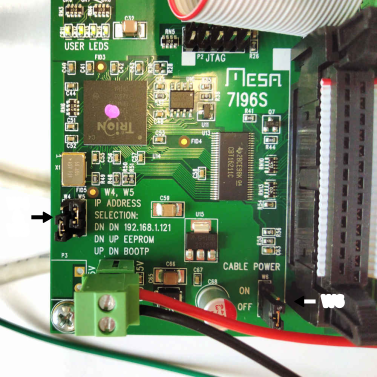
\includegraphics[width=1\linewidth]{images/mesa/mesa_7i96s_bottom_left_labelled.pdf}
    \caption{Vista de la parte inferior izquierda de la placa MESA 7I96S.}
    \label{fig:mesa_ip_selection}
\end{figure}

Las opciones de configuración de IP disponibles se detallan en la \cref{tab:mesa_ip_selection}. En particular cabe destacar lo siguiente:
\begin{itemize}
    \item Con los jumpers W4 y W5 en la posición (abajo, arriba) la dirección IP se leerá de la EEPROM. La dirección IP de serie en la EEPROM es 10.10.10.10. Esta dirección IP se puede cambiar mediante la utilidad \texttt{mesaflash}, por ejemplo para establecer la IP en la EEPROM a 10.10.10.100 ejecutaríamos el siguiente comando:
    %
\begin{listingbox}
mesaflash --device 7i96s --addr 192.168.1.121 --set ip=10.10.10.100
\end{listingbox}

    \item Con los jumpers W4 y W5 en la posición (arriba, arriba) la direción IP se establecerá a 192.168.1.121 y la placa arrancará usando la configuración de respaldo (ver \cref{sec:mesa7i96s_fallback}).
\end{itemize}


\begin{table}[!ht]
    \centering
    \begin{tabular}{lll}
        \toprule
        W4 & W5 & Dirección IP \\
        \midrule
        Abajo  & Abajo  & 192.168.1.121 \\
        Abajo  & Arriba & Leída de la EEPROM \\
        Arriba & Abajo  & Obtenida vía BOOTP \\
        Arriba & Arriba & 192.168.1.121 y usar conf. de respaldo \\
        \bottomrule
    \end{tabular}
    \caption{Opciones de configuración de la dirección IP en la placa MESA 7I96S mediante los jumpers W4 y W5.}
    \label{tab:mesa_ip_selection}
\end{table}


En el montaje de prueba se han establecido los jumpers W4 y W5 en la posición (abajo, arriba) como se muestra en la \cref{fig:mesa_ip_selection}. De esta forma la placa lee la dirección IP grabada en la EEPROM. En este caso hemos establecido la dirección IP de la placa a 10.68.33.122.


\subsubsection{Configuración de respaldo}
\label{sec:mesa7i96s_fallback}

La memoria flash de la placa MESA 7I96S contiene dos imágenes, una principal, y otra de respaldo. Si la imagen primaria se corrompe, la FPGA cargará la configuración de respaldo, de esta forma se podrá grabar una nueva imagen principal. De otra forma habría que programar la memoria mediante JTAG.

Se puede forzar a que la placa arranque usando la configuración de respaldo estableciendo los jumpers de selección de IP W4 y W5 a la posición (arriba,arriba). Con este modo de arranque la dirección IP de la tarjeta se establecerá a 192.168.1.121.


\subsubsection{Alimentación de \qty{5}{\V} del conector de expansión}
\label{sec:mesa7i96s_cable_power}

La placa MESA 7I96S tiene la opción de suministrar alimentación de 5V a la placa conectada a su conector de expansión (P1), en nuestro caso la MESA 7I77. Esta opción esta controlada por el jumper W6, situado en la parte inferior de la placa a la izquierda del conector de expansión, como se muestra en la \cref{fig:mesa_ip_selection}, de forma que:
%
\begin{itemize}
    \item Con el jumper W6 en la posición arriba, la placa MESA 7I96S proporcionará alimentación a la placa MESA 7I77 a través del conector de expansión.

    \item Con el jumper W6 en la posición abajo, la placa MESA 7I96S no proporcionará alimentación a través del conector de expansión, deberemos proporcionar alimentación externa a la placa MESA 7I77.
\end{itemize}


% En la \cref{tab:mesa7i96s_cable_power} se indican las configuraciones posibles.

% \begin{table}[!ht]
%     \centering
%     \begin{tabular}{ll}
%         \toprule
%         W6 & Alimentación \\
%         \midrule
%         Arriba & Activada \\
%         Abajo  & Desactivada \\
%         \bottomrule
%     \end{tabular}
%     \caption{Opciones de configuración de la alimentación de \qty{5}{\V} del conector de expansión.}
%     \label{tab:mesa7i96s_cable_power}
% \end{table}

% Configurando el jumper W6 en la posición arriba, la placa MESA 7I77 obtendrá se alimentación principal a través de la MESA 7I96S. Si configuramos el jumper W6 en la posición abajo, deberemos proporcionar alimentación externa a la placa MESA 7I77.

En el montaje de prueba se ha escogido esta última opción, configurando el jumper W6 en la posición abajo, como puede verse en la \cref{fig:mesa_ip_selection}. La placa MESA 7I77 también deberá configurarse adecuadamente como se explica en la \cref{sec:mesa7i77_power}.


\subsection{Configuración de la placa MESA 7I77}

\subsubsection{Alimentación principal de \qty{5}{\V}}
\label{sec:mesa7i77_power}

La placa MESA 7I77 puede obtener su alimentación principal a través de la placa MESA 7I96S, o a través de su conector TB1. Esta alimentación debe ser de \qty{5}{\V} y se usa para alimentar los encoders, las salidas analógicas, y la interfaz RS-422. El modo de la alimentación principal en la MESA 7I77 se selecciona mediante el jumper W5 de la siguiente forma:
%
\begin{enumerate}
    \item Si W5 está en la posición izquierda, la alimentación se obtiene a través de la placa MESA 7I96S, en este caso el jumper W6 de la placa MESA 7I96S deberá establecerse en la posición arriba.

    \item Si W5 está en la posición derecha, se debe suministrar la alimentación a la placa mediante el conector TB1, en este caso el jumper W6 de la placa MESA 7I96S deberá establecerse en la posición abajo para que no proporcione energía a la placa hija.
\end{enumerate}

\begin{admonition}{Importante}
    Suministrar alimentación a la placa MESA 7I77 a través del conector TB1 con el jumper W5 en la posición izquierda puede dañar la placa MESA 7I77, la placa MESA 7I96S, el cable de conexión, e incluso el PC.
\end{admonition}

En el montaje de prueba se ha escogido alimentar a la placa MESA 7I77 a través del conector TB1, por lo que:
\begin{itemize}
    \item El jumper W6 de la placa MESA 7I96S se ha establecido en la posición abajo. Esto se puede ver en la \cref{fig:mesa_ip_selection}.
    
    \item El jumper W5 de la placa MESA 7I77 se ha establecido en la posición derecha. Esto se muestra en la \cref{fig:mesa7i77_left}.
\end{itemize}


\begin{figure}[!ht]
    \centering
    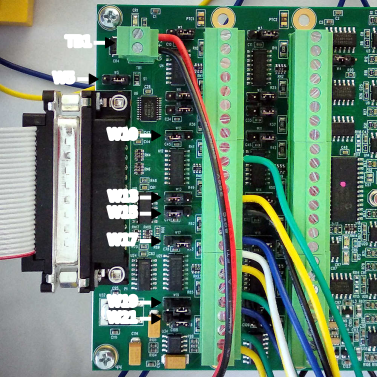
\includegraphics[width=1\linewidth]{images/mesa/mesa_7i77_left_labelled.pdf}
    \caption{Vista de la parte izquierda de la placa MESA 7I77.}
    \label{fig:mesa7i77_left}
\end{figure}


\subsubsection{Alimentación de las entradas y salidas digitales}

Aparte de la alimentación principal de \qty{5}{\V}, la placa MESA 7I77 también necesita alimentación adicional para las entradas y salidas digitales a través del conector TB2 (ver \cref{fig:installation,fig:mesa7i77_right}). El listado de conexiones del conector TB2 se reproduce en la \cref{tab:mesa7i77_tb2}.

\begin{table}[!ht]
    \centering
    \begin{tabular}{lll}
        \toprule
        Pin & Señal & Función \\
        \midrule
        1 (abajo)  & VFIELD & FIELD POWER \\
        2          & VFIELD & FIELD POWER \\
        3          & VFIELD & FIELD POWER \\
        4          & VFIELD & FIELD POWER \\
        5          & VIN    & FIELD I/O LOGIC POWER \\
        6          & No conectado \\
        7          & No conectado \\
        8 (arriba) & Tierra & Referencia de VIN \& VFIELD \\
        \bottomrule
    \end{tabular}
    \caption{Conexiones del conector TB2 de la placa MESA 7I77.}
    \label{tab:mesa7i77_tb2}
\end{table}

Como se puede ver en la \cref{tab:mesa7i77_tb2}, en este caso la placa requiere de dos entradas de alimentación:
\begin{itemize}
    \item \textbf{VFIELD}: Esta entrada proporciona la alimentación de las salidas y determina los niveles lógicos de las entradas. Entre \qtyrange[range-phrase={ y }]{5}{28}{\V}.
    \item \textbf{VIN}: La alimentación para la lógica de las entradas y salidas. Entre \qtyrange[range-phrase={ y }]{8}{32}{\V}.
\end{itemize}

Si VFIELD está entre \qtyrange[range-phrase={ y }]{8}{28}{\V}, puede usarse la misma fuente para alimentar a VIN. Para esto la placa incluye el jumper W1, que al colocarlo en la posición izquierda conecta VIN con VFIELD. Si queremos usar valores de VFIELD fuera del rango de VIN, por ejemplo, \qty{5}{\V}, debemos colocar W1 en la posición derecha para desconectar VIN e VFIELD, de esta forma podemos usar fuentes de alimentación separadas para VIN y VFIELD.

\begin{admonition}{Importante}
    La tensión en VFIELD debe tener una tasa de aumento máxima de \qty{10}{\V/\m\s}, de lo contrario la placa puede sufrir daños. Esta es una limitación de los transistores MOSFET \cite{toshiba2018impacts, toshiba2018mosfets, nexperia2023power, bai2003analysis}. Por lo tanto, VFIELD debe conectarse directamente a la fuente de alimentación sin usar interruptores, disyuntores, o contactos de relé en el circuito. Un fusible es aceptable pero en ningún caso debe conectarse VFIELD a través de un contacto mecánico.
\end{admonition}

Como se comentó en la \cref{sec:page_input_outputs}, la placa MESA 7I96S solamente puede usar lógica de \qty{5}{\V} para las señales de paso y dirección, y por lo tanto, la lógica de los controladores Igus dryve D1 y de la placa MESA 7I77 debe ser también a \qty{5}{\V}. De esta forma, en el montaje de prueba se ha establecido en la placa MESA 7I77 el jumper W1 en la posición derecha, la entrada VIN a \qty{24}{\V}, y la entrada VFIELD a \qty{5}{\V}. Esto se muestra en la \cref{fig:mesa7i77_right}.


\begin{figure}[!ht]
    \centering
    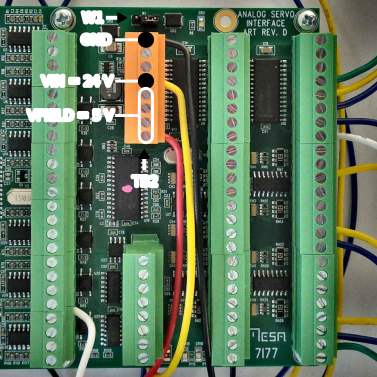
\includegraphics[width=1\linewidth]{images/mesa/mesa_7i77_right_labelled.pdf}
    \caption{Vista de la parte derecha de la placa MESA 7I77.}
    \label{fig:mesa7i77_right}
\end{figure}


\subsubsection{Modos de entrada de los encoders}

La placa MESA 7I77 dispone de seis entradas para encoders, cada una con entradas individuales A, B, y Z. Estas entradas pueden configurarse para funcionar con señales diferenciales o con señales de terminación única. Cada encoder dispone de 3 jumpers para configurar el modo de las entradas individuales A, B, y Z. En la posición derecha se selecciona el modo diferencial, y en la posición izquierda el modo de terminación única. El listado de jumpers para las entradas individuales de cada encoder se muestra en la \cref{tab:encoder_jumpers}.

\begin{table}[!ht]
    \centering
    \begin{tabular}{llll}
        \toprule
        Encoder & \multicolumn{3}{c}{Jumpers} \\
        \cmidrule{2-4}
        & A & B & Z \\
        \midrule
        0 & W21 & W19 & W17 \\
        1 & W15 & W13 & W10 \\
        2 & W8  & W6  & W2 \\
        3 & W22 & W20 & W18 \\
        4 & W16 & W14 & W11 \\
        5 & W9  & W7  & W3 \\
        \bottomrule
    \end{tabular}
    \caption{Jumpers de configuración de los encoders.}
    \label{tab:encoder_jumpers}
\end{table}

En el montaje de prueba se usaron las siguientes entradas y modos de encoder de la placa MESA 7I77:
\begin{itemize}
    \item En la entrada 0 se conectó el encoder del motor paso a paso. Este encoder es de señal diferencial, por lo que los jumpers W21, W19, y W17 se dejaron en la posición derecha, esta es la posición de serie.

    \item En la entrada 1 se conectó el encoder del motor sin escobillas. Este encoder es de señal de terminación única, por lo que en este caso se establecieron los jumpers W15, W13, y W10 en la posición izquierda. 
\end{itemize}

La configuración de los jumpers anteriormente citados para los encoders 0 y 1 de la placa MESA 7I77 en el montaje de prueba se muestra en la \cref{fig:mesa7i77_left}.


\subsection{Introducción a LinuxCNC}

LinuxCNC es un conjunto de aplicaciones altamente personalizables para el control máquinas de \ac{CNC}, impresoras 3D, robots, y otros dispositivos automatizados. Es capaz de proporcionar control coordinado de hasta 9 ejes de movimiento. LinuxCNC consta de varios componentes clave que están integrados para formar un sistema completo \cite{linuxcncdoc}:

\begin{itemize}
    \item Una \ac{GUI}, que constituye la interfaz básica entre el operador, el software, y la máquina \ac{CNC} en sí misma.
    
    \item La \acf{HAL}, que permite enlazar las señales del mundo exterior con LinuxCNC y viceversa.
    
    \item Los módulos de alto nivel que coordinan la generación, ejecución, y control de movimiento de la máquina \ac{CNC}, a saber, el controlador de movimiento, el controlador de entrada/salida, y el ejecutor de tareas.
\end{itemize}

En este documento se proporciona solo una pequeña guía de LinuxCNC, para más detalles se recomienda consultar el manual de usuario de LinuxCNC \cite{linuxcncdoc}, en donde se detalla ampliamente como usar el software. En un sistema con LinuxCNC instalado, el manual se puede consultar haciendo clic en \menu{Applications menu > CNC > Documentation > User Manual - EN}.


\subsubsection{Ejecutar LinuxCNC}

Podemos ejecutar LinuxCNC haciendo clic en \menu{Applications menu > CNC > LinuxCNC} o mediante el comando \texttt{linuxcnc}, cuya forma de uso se muestra en el \cref{lst:linuxcnc_help}.

\begin{listingtitledbox}[
    title=Uso del comando \texttt{linuxcnc},
    label=lst:linuxcnc_help,
][
    basicstyle=\ttfamily\footnotesize,
]
linuxcnc: Run LinuxCNC

Usage:
  $ linuxcnc -h
    This help

  $ linuxcnc [Options]
    Choose the configuration INI file graphically

  $ linuxcnc [Options] path/to/your_ini_file
    Name the configuration INI file using its path

  $ linuxcnc [Options] -l
    Use the previously used configuration INI file

Options:
    -d: Turn on "debug" mode
    -v: Turn on "verbose" mode
    -r: Disable redirection of stdout and stderr to ~/linuxcnc_print.txt and
        ~/linuxcnc_debug.txt when stdin is not a tty.
        Used when running linuxcnc tests non-interactively.
    -l: Use the last-used INI file
    -k: Continue in the presence of errors in HAL files
    -t "tpmodulename [parameters]"
            specify custom trajectory_planning_module
            overrides optional INI setting [TRAJ]TPMOD
    -m "homemodulename [parameters]"
            specify custom homing_module
            overrides optional INI setting [EMCMOT]HOMEMOD
    -H "dirname": search dirname for HAL files before searching
                  INI directory and system library:
                  /home/git/linuxcnc-dev/lib/hallib
Note:
    The -H "dirname" option may be specified multiple times
\end{listingtitledbox}

Si hacemos clic en \menu{Applications menu > CNC > LinuxCNC} o ejecutamos el comando \texttt{linuxcnc} sin pasarle como parámetro un archivo de configuración se abrirá el selector de configuración de LinuxCNC, como se muestra en la \cref{fig:linuxcnc_conf_selector}.

\begin{figure}[!ht]
    \centering
    \includegraphics[width=\linewidth]{images/linuxcnc/configuration_selector.png}
    \caption{Selector de configuración de LinuxCNC}
    \label{fig:linuxcnc_conf_selector}
\end{figure}

En el selector de configuración se muestran las configuraciones disponibles en una estructura de árbol, reflejando la estructura de directorios donde se almacenan, con dos nodos iniciales:
%
\begin{itemize}
    \item \textbf{My configurations}: configuraciones del usuario, almacenadas en la carpeta \path{~/linuxcnc/configs}.
    
    \item \textbf{Sample configurations}: configuraciones de ejemplo proporcionadas de serie con LinuxCNC. Estas se almacenan en \path{/usr/share/doc/linuxcnc/examples/sample-configs}.
\end{itemize}

Al hacer clic en una de las configuraciones se mostrará su información en el recuadro derecho de la aplicación. Para arrancar LinuxCNC con una configuración simplemente hay que hacer doble clic en ella o seleccionarla y pulsar el botón \button{OK}. Si marcamos la casilla «Create Desktop Shortcut», se creará además un icono en el escritorio para lanzar directamente LinuxCNC con la respectiva configuración. Por último, si la configuración es una de las de \textit{Sample configurations}, LinuxCNC preguntará al usuario si copiarla a la carpeta \path{~/linuxcnc/configs}, de forma que el usuario pueda modificarla posteriormente. En caso de responder afirmativamente, posteriormente la configuración aparecerá dentro de la categoría \textit{My configurations}.


\subsubsection{Archivos de configuración}
\label{sec:linuxcnc_intro_config}

Una configuración de LinuxCNC se compone de varios archivos. Por ejemplo, considerando una carpeta de configuración con nombre «robot», para una configuración típica tendríamos los siguientes archivos:
%
\begin{itemize}
    \item \texttt{robot.ini}: Configuración principal de LinuxCNC. Aquí se definen parámetros como velocidades, aceleraciones, configuración de ejes, y otros ajustes importantes.

    \item \texttt{robot.hal}: Archivo principal de la \acf{HAL}. Contiene la configuración de la asignación de señales de LinuxCNC con la interfaz de hardware del sistema. Define cómo los componentes físicos se relacionan con las señales lógicas dentro de LinuxCNC. Al iniciar LinuxCNC, este archivo se lee y se procesa antes de que se cargue la \ac{GUI}.

    \item \texttt{robot\_custom.hal} (opcional): LinuxCNC permite especificar varios archivos \texttt{.hal}. Este archivo contendrá  configuraciones adicionales de la \acl{HAL}.

    \item \texttt{robot\_postgui.hal} (opcional): Configuraciones de la \acl{HAL} que se realizarán después de que la \ac{GUI} se haya cargado. Esto puede incluir configuraciones de visualización como por ejemplo enlazar una señal de LinuxCNC con un elemento de la \ac{GUI} para mostrar su valor.

    \item \texttt{rs274ngc.var} (opcional): Parámetros para el intérprete de G-code (ver \cref{sec:linuxcnc_intro_gcode}) que serán persistentes entre distintas ejecuciones de LinuxCNC.

    \item \texttt{tool.tbl} (opcional): Configuración de la tabla de herramientas. Se utiliza para definir herramientas y sus propiedades, como dimensiones y compensaciones. Es importante para el sistema saber exactamente cómo está configurada cada herramienta para realizar operaciones precisas en las piezas de trabajo.
\end{itemize}

En la \cref{sec:linuxcnc_configuration} se muestra un ejemplo de configuración de LinuxCNC.


\subsubsection{Lenguaje G-code}
\label{sec:linuxcnc_intro_gcode}

El G-code es el lenguaje de programación más usado en \ac{CNC}. Un programa G-code consiste en una serie de instrucciones que indica a la máquina cómo moverse o cómo realizar operaciones específicas. El G-code tiene sus raíces en los primeros días de la automatización industrial. Se desarrolló como una forma estándar de comunicar instrucciones a las máquinas \ac{CNC} en los años 50 y 60. Se estandarizó como RS-274 por la \ac{EIA} en 1963, y su revisión final se estandarizó como RS-274-D en 1979 y como ISO 6984 en 1982. Posteriormente, surgieron numerosas implementaciones y estándares derivados, desarrollados tanto por organismos públicos como privados.

En LinuxCNC, el G-code es el lenguaje que se utiliza para controlar el movimiento de la máquina. En particular, la versión implementada por LinuxCNC se basa en el lenguaje RS274/NGC desarrollado por el \ac{NIST} \cite{RS274NGC}. En la documentación de LinuxCNC se documenta ampliamente el lenguaje G-code \cite[sección G-code Programming]{linuxcncdoc}. Como ejemplo, a continuación se presentan algunos comandos de G-code.
%
\begin{itemize}
    \item \texttt{G0 X10 Y5 Z3}: Movimiento rápido a las coordenadas X=10, Y=5, y Z=3.
    \item \texttt{F100}: Establece el \textit{feed rate} (velocidad de movimiento) a 100 unidades por minuto.
    \item \texttt{G1 X20 Y15}: Movimiento a las coordenadas X=20 e Y=15 a la velocidad establecida en el \textit{feed rate}.
    \item \texttt{G1 F100 X20 Y15}: Establece el \textit{feed rate} a 100 unidades por minuto y realiza un movimiento a las coordenadas X=20 e Y=15.
    \item \texttt{G2 X30 Y10 I5 J0}: Movimiento circular en sentido horario con centro en X=5, Y=0 y radio de 5 unidades.
    \item \texttt{G3 X40 Y5 I2 J3}: Movimiento circular en sentido antihorario con centro en X=2, Y=3 y radio de 5 unidades.
    \item \texttt{M3 S1000}: Encender el husillo a \qty{1000}{rpm} en sentido horario.
    \item \texttt{M5}: Apagar el husillo.
\end{itemize}

Estos son solo algunos ejemplos básicos de comandos G-code. En la práctica, los programas G-code se compondrán de varias líneas, cada una con un comando, y como cualquier otro lenguaje de programación podrán definir variables, subrutinas, y usar bucles o control de flujo.


\subsubsection{Modos de operación}
\label{sec:linuxcnc_modes_of_operation}

En LinuxCNC hay tres modos de operación, cada uno diseñado para un propósito específico: manual, automático, y \ac{MDI}. Estos modos definen cómo se ingresan y ejecutan los comandos, y cada uno tiene sus propias características distintivas:
%
\begin{itemize}
    \item En el modo manual, los comandos se ingresan individualmente. Estos comandos son acciones directas, como «activar refrigerante» o «mover el eje X a 25 pulgadas por minuto». En las de interfaces gráficas se maneja normalmente mediante botones o atajos de teclado.

    \item El modo automático permite la ejecución completa de programas G-code almacenados en archivos. Un único comando puede cargar y ejecutar un archivo entero.

    \item El modo \ac{MDI} permite ejecutar comandos individuales de G-code.
\end{itemize}

Es importante tener en cuenta que ciertos comandos, como \textit{Abort}, \textit{Emergency Stop}, y \textit{Feed Rate Override}, pueden usarse en todos los modos. 


\subsubsection{Interfaz gráfica}

LinuxCNC proporciona diversas interfaces gráficas para controlar las máquinas \ac{CNC}. La interfaz específica a usar se configura en el archivo \texttt{.ini}. La lista completa de interfaces gráficas disponibles con imágenes y ejemplos se puede consultar en el manual de usuario de LinuxCNC \cite{linuxcncdoc}.

Una de las interfaces gráficas más populares es «AXIS», pensada para ser controlada mediante teclado y ratón. Esta interfaz gráfica se muestra en la \cref{fig:linuxcnc_gui_axis_estop}. Por otra parte, LinuxCNC también dispone de la interfaz «HALUI», una interfaz puramente hardware, que permite controlar la máquina \ac{CNC} solamente usando botones e interruptores físicos.
%
\begin{figure}[!ht]
    \centering
    \includegraphics[width=\linewidth]{images/linuxcnc/linuxcnc_gui_axis.png}
    \caption{Interfaz gráfica «AXIS» de LinuxCNC.}
    \label{fig:linuxcnc_gui_axis_estop}
\end{figure}

En el montaje de prueba hemos considerado la interfaz gráfica AXIS. La ventana de esta interfaz, como se muestra en la \cref{fig:linuxcnc_gui_axis_estop}, contiene los siguientes elementos:
\begin{itemize}
    \item Un área de visualización con dos pestañas:
    \begin{itemize}
        \item Pestaña «Preview»: muestra la posición del punto controlado por la máquina. Posteriormente, mostrará la ruta trazada por la máquina.

        \item Pestaña «DRO» (\acl{DRO}): muestra la posición actual y todas las compensaciones.
    \end{itemize}

    \item Una barra de menú y una barra de herramientas que permiten realizar diversas acciones.
    
    \item Pestaña «Manual Control»: permite mover la máquina.

    \item Pestaña «MDI» (\acl{MDI}): permite introducir programas de G-code manualmente, línea a línea.
    
    \item «Feed Override»: permite escalar la velocidad de los movimientos programados.

    \item «Rapid Override»: permite escalar la velocidad de los movimientos rápidos (e.g., códigos \texttt{G0} de G-code).
    
    \item «Jog Speed»: permite configurar la velocidad de «jog», i.e., la velocidad cuando se controla el robot con los controles \button{-} y \button{+} de la pestaña «Manual Control».
    
    \item «Max Velocity»: permite limitar la velocidad máxima de todos los movimientos programados.
    
    \item «Active G-codes»: muestra los códigos G modales que están vigentes. Algunos de los más relevantes de los que se muestran en la \cref{fig:linuxcnc_gui_axis_estop} son:
    \begin{itemize}
        \item \texttt{G17}: Establece el plano de trabajo de la máquina en XY. 
        
        \item \texttt{G21}: Establece las unidades de medida en milímetros.

        \item \texttt{G90}: Establece la modalidad de coordenadas absolutas.

        \item \texttt{G94}: Establece que el «feed rate» (velocidad de avance) se interpretará en unidades por minuto.

        \item \texttt{F0}: Establece el «feed rate» (velocidad de avance) en cero.
    \end{itemize}

    La información detallada de los códigos G se puede consultar en el manual de usuario de LinuxCNC \cite[sección G-Codes]{linuxcncdoc}, también disponible en \url{https://linuxcnc.org/docs/html/gcode/g-code.html}.

    \item Un área de visualización de texto que muestra el archivo de G-code cargado.
    
    \item Una barra de estado que muestra distintos datos de utilidad: 
    \begin{itemize}
        \item El estado de la máquina: «ESTOP» (parada de emergencia), «OFF» (apagada), o «ON» (encendida).

        \item La herramienta insertada.

        \item La posición mostrada: «relative» (mostrando todas las compensaciones), o «actual» (mostrando la posición de retroalimentación).
    \end{itemize}
\end{itemize}


\subsection{Uso básico de LinuxCNC}
\label{sec:linuxcnc_usage}

Durante el desarrollo del montaje de prueba se han elaborado tres configuraciones principales de LinuxCNC:
%
\begin{itemize}
    \item \texttt{mesa\_7i96s\_7i77\_xy}: Simula un robot con ejes X e Y, donde el motor sin escobillas controla el eje X, y el motor paso a paso el eje Y.

    \item \texttt{mesa\_7i96s\_7i77\_xx}: Simula un robot con un único eje X, donde ambos motores, sin escobillas y paso a paso, controlan al mismo tiempo el eje. Por lo tanto, en este caso ambos motores se mueven síncronamente a la misma velocidad.

    \item \texttt{mesa\_7i96s\_7i77\_xc}: Simula un robot con un eje X y un eje C, siendo el eje C el de rotación alrededor del eje Z. El motor sin escobillas controla el eje X, y el motor paso a paso el eje C.
\end{itemize}

En las siguientes secciones se explica como usar LinuxCNC con estas configuraciones.


\subsubsection{Control mediante la interfaz gráfica AXIS}
\label{sec:linuxcnc_usage_gui_axis}

Al arrancar LinuxCNC con una de las configuraciones anteriores se abrirá la interfaz gráfica AXIS como se muestra en la \cref{fig:linuxcnc_gui_axis_estop}. A continuación se explica el proceso para controlar la máquina con esta interfaz.

\paragraph{Establecer el estado de LinuxCNC a «ON»}\hfill\medskip

El estado inicial de LinuxCNC será «ESTOP» (parada de emergencia), como se indica en la parte inferior izquierda de la ventana, y por lo tanto el movimiento del robot estará deshabilitado. Para poder arrancar el robot en primer lugar deberemos eliminar la condición de «ESTOP». para esto hacemos lo siguiente:
%
\begin{enumerate}
    \item Desactivar el interruptor físico de parada de emergencia (ver \cref{fig:installation}). Si este interruptor está activado se fuerza el estado de parada de emergencia en LinuxCNC.

    \item Desactivar el estado de parada de emergencia en LinuxCNC pulsando el botón \graphicbutton{images/linuxcnc/linuxcnc_gui_axis_button_estop.png}.
\end{enumerate}

Una vez desactivado el estado de parada de emergencia, LinuxCNC pasará al estado «OFF» (apagado) y el botón de arranque pasará de desactivado: \graphicbutton{images/linuxcnc/linuxcnc_gui_axis_button_on_disabled.png} a activado: \graphicbutton{images/linuxcnc/linuxcnc_gui_axis_button_on.png}. Para empezar a usar el robot pulsaremos este botón, de esta forma LinuxCNC pasará al estado «ON» (encendido). En la \cref{fig:linuxcnc_gui_axis_on} se muestra la interfaz AXIS en el estado «ON».

\begin{figure}[!ht]
    \centering
    \includegraphics[width=\linewidth]{images/linuxcnc/linuxcnc_gui_axis_on.png}
    \caption{Interfaz gráfica «AXIS» de LinuxCNC en estado «ON».}
    \label{fig:linuxcnc_gui_axis_on}
\end{figure}


\paragraph{Referenciar la máquina}\hfill\medskip

Una vez que LinuxCNC está en estado «ON», podemos controlar manualmente la máquina a través de los controles \button{-} y \button{+} de la pestaña «Manual Control». Sin embargo, para ejecutar comandos específicos de posicionamiento de G-code, e.g., mover la máquina a (X=1, Y=5), es necesario llevar a cabo el proceso de «homing» o referenciación de la máquina. El procedimiento de «homing» implica establecer un punto de referencia preciso para todos los ejes de la máquina, de forma que LinuxCNC tenga conocimiento exacto de la posición de la máquina.

Para realizar el proceso de «homing» podemos hacer clic en el botón \button{Home All} de la pestaña «Manual Control» o en la entrada de menú \menu{Machine > Homing > Home all axes}. En las configuraciones de prueba el proceso de «homing» involucra el uso de los interruptores de límite. El proceso que sigue LinuxCNC para realizar el «homing» mediante interruptores de límite es el siguiente:
\begin{enumerate}
    \item Mover el motor hacia el interruptor de límite hasta encontrarlo, i.e., activarlo.

    \item Mover el motor en sentido opuesto hasta desactivar el interruptor de límite.

    \item Mover el motor otra vez hacia el interruptor de límite hasta encontrarlo, esta vez a una velocidad inferior para localizar la posición del interruptor de forma precisa.

    \item Mover el motor hasta la posición de referencia «home».
\end{enumerate}
%
En las configuraciones \texttt{mesa\_7i96s\_7i77\_xy} y \texttt{mesa\_7i96s\_7i77\_xx} deberemos activar manualmente los interruptores de límite para ambos motores. En la configuración \texttt{mesa\_7i96s\_7i77\_xc} solo deberemos activar manualmente el interruptor de límite para el motor sin escobillas, el motor paso a paso en este caso usa un proceso de «homing» distinto que simplemente busca la posición del pulso de índice del encoder.

En la figura \cref{fig:linuxcnc_gui_axis_on_homed} se muestra la ventana de la interfaz después de completar el proceso de referenciado. Ahora se puede ver el símbolo \smash{\raisebox{-0.2\baselineskip}{\includegraphics[height=0.8\baselineskip]{images/linuxcnc/linuxcnc_gui_axis_homed_symbol.png}}} al lado de la información de los ejes X e Y en el área de visualización, lo que indica que los ejes están referenciados.

\begin{figure}[!ht]
    \centering
    \includegraphics[width=\linewidth]{images/linuxcnc/linuxcnc_gui_axis_on_homed.png}
    \caption{Interfaz gráfica «AXIS» de LinuxCNC en estado «ON» y con todos los ejes referenciados.}
    \label{fig:linuxcnc_gui_axis_on_homed}
\end{figure}


\paragraph{Controlar la máquina}\hfill\medskip

Como se comentó en la \cref{sec:linuxcnc_modes_of_operation}, LinuxCNC dispone de 3 modos de control: manual, \ac{MDI}, y automático. La interfaz AXIS permite controlar la máquina con estos modos de la siguiente forma:
\begin{itemize}
    \item \textbf{Modo manual}: podemos controlar la máquina en modo manual a través de los controles \button{-} y \button{+} de la pestaña «Manual Control».

    \item \textbf{Modo \acs{MDI}}: podemos usar el modo \ac{MDI} a través de la pestaña «MDI», donde se pueden introducir comandos G-code línea a línea.

    \item \textbf{Modo automático}: podemos cargar un programa de G-code en archivo haciendo clic en \menu{File > Open} y a continuación ejecutarlo en modo automático haciendo clic en el botón \graphicbutton{images/linuxcnc/linuxcnc_gui_axis_button_run.png} o pulsando la tecla \keys{R}.
\end{itemize}

Para más información acerca del control mediante G-code consultar la sección «G-code programming» en el manual de LinuxCNC \cite{linuxcncdoc}.


\subsubsection{Control programado}

Podemos controlar LinuxCNC mediante programas que incluyan una secuencia de instrucciones de las siguientes dos formas:
%
\begin{enumerate}
    \item Usando programas de G-code en archivo como se comentó en la sección anterior.

    \item Usando programas en Python utilizando la biblioteca \texttt{linuxcnc}, incluida con LinuxCNC, que permite interactuar con el proceso en ejecución de LinuxCNC. Para más información consultar la sección «Python Interface» en el manual de usuario de LinuxCNC. En el \cref{lst:linuxcnc_python} se muestra un ejemplo de control del robot con Python mediante el envío de comandos G-code en modo \ac{MDI}.
\end{enumerate}


\begin{listingtitledbox}[
    title=Ejemplo de uso de Python para interactuar con LinuxCNC,
    label=lst:linuxcnc_python,
][
    basicstyle=\ttfamily\footnotesize,
    language=Python,
]
#!/usr/bin/env python3
# Example of LinuxCNC control with Python
# See the LinucCNC user manual, section 13.5 - Python Interface

import sys
import linuxcnc


def control_robot(c: linuxcnc.command) -> None:
    def set_feed_rate(v: float):
        # set robot feed rate
        c.mdi(f"F{v}")
        c.wait_complete()

    def go_to(x: float, y: float):
        # go to position (x, y)
        print(f"Going to ({x}, {y})...", end="", flush=True)
        c.mdi(f"G1 X{x} Y{y}")
        while (ret := c.wait_complete(1)) == -1:
            continue
        print(" done")
        if ret == linuxcnc.RCS_ERROR:
            print("RCS_ERROR")

    # Put your robot commands here
    set_feed_rate(400)
    go_to(0, 0)


def main():
    s = linuxcnc.stat()  # connect to the status channel
    c = linuxcnc.command()  # connect to the command channel

    def ok_for_mdi() -> bool:
        s.poll()
        return (
            not s.estop
            and s.enabled
            and (s.homed.count(1) == s.joints)
            and (s.interp_state == linuxcnc.INTERP_IDLE)
        )

    if ok_for_mdi():
        c.mode(linuxcnc.MODE_MDI)
        c.wait_complete()  # wait until mode switch executed
        print("OK, running...")
        try:
            control_robot(c)
        except KeyboardInterrupt:
            c.abort()
            sys.exit(1)
    else:
        print("Not OK for running. Check that the robot is homed and idle.")
        sys.exit(1)


if __name__ == "__main__":
    try:
        main()
    except linuxcnc.error as e:
        print("error: ", e)
        print("is LinuxCNC running?")
        sys.exit(1)
\end{listingtitledbox}


\subsection{Configuración de LinuxCNC}
\label{sec:linuxcnc_configuration}

Como se comentó en la \cref{sec:linuxcnc_intro_config}, una configuración de LinuxCNC se compone de varios archivos, siendo necesarios por lo menos un archivo INI y un archivo HAL. En las siguientes secciones se explica la configuración de ambos tipos de archivo, usando como ejemplo la configuración de prueba \texttt{mesa\_7i96s\_7i77\_xy}.


\subsubsection{Configuración INI}
\label{sec:linuxcnc_configuration_ini}

\paragraph{Formato de archivo de configuración .ini}\hfill\medskip

Un archivo \texttt{.ini} es un archivo de texto plano que se utiliza para configurar aplicaciones y programas. Tiene una estructura sencilla que consiste en secciones y claves con sus respectivos valores. A continuación, se describe la sintaxis básica de un archivo \texttt{.ini}:

\begin{itemize}
    \item \textbf{Secciones}:
    Las secciones se utilizan para organizar las claves y valores. Cada sección comienza con el nombre de sección entre corchetes, seguido de cero o más pares clave-valor que pertenecen a esa sección. La sintaxis para una sección es la siguiente:

\begin{listingbox}[][language=ini]
[nombre_de_seccion]
\end{listingbox}

    \item \textbf{Claves y Valores}:
    Dentro de cada sección se pueden definir claves y sus valores correspondientes. Las claves son identificadores que se utilizan para acceder a los valores asociados. La sintaxis para una clave y su valor es la siguiente:

\begin{listingbox}[][language=ini]
clave = valor
\end{listingbox}

    Las claves pueden contener letras y guiones bajos (\_). Los valores pueden ser cadenas de texto, números enteros o números de punto flotante.

    \item \textbf{Comentarios}:
    Los comentarios comienzan con el símbolo de punto y coma (;) o el símbolo de almohadilla (\#). Por ejemplo:

\begin{listingbox}[][language=ini]
; Esto es un comentario
# Esto también es un comentario
\end{listingbox}
\end{itemize}


\paragraph{Ejemplo: archivo de configuración \texttt{mesa\_7i96s\_7i77\_xy.ini}}\hfill\medskip

A continuación se muestran las distintas secciones del archivo de configuración \texttt{mesa\_7i96s\_7i77\_xy.ini}, donde los distintos parámetros de cada sección aparecen comentados explicando para que sirven. En algunas secciones no se han especificado todos los parámetros disponibles, para ver la lista completa de parámetros y su documentación consultar el manual de usuario de LinuxCNC \cite{
linuxcncdoc}.

\begin{itemize}
    \item \textbf{Sección EMC}: Configuración general
    %
    \inilistingbox[][linerange=1-12]{codes/mesa_7i96s_7i77_xy.ini}

    \item \textbf{Sección DISPLAY}: Configuración de la interfaz de usuario. Las opciones disponibles pueden depender de la interfaz de usuario que se use. En este caso usamos la interfaz de usuario AXIS.
    %
    \inilistingbox[][linerange=15-65]{codes/mesa_7i96s_7i77_xy.ini}

    \item \textbf{Sección TASK}: Configuración del controlador de tareas de LinuxCNC. El controlador de tareas se encarga de comunicarse con la interfaz de usuario, comunicarse con el planificador de movimiento, y
    comunicarse con el interprete de G-code. Actualmente solo existe un controlador de tareas, \texttt{milltask}. Para más información consultar el manual de usuario de LinuxCNC \cite{linuxcncdoc} y la página de manual de \texttt{milltask}, también disponible en \url{http://linuxcnc.org/docs/devel/html/man/man1/milltask.1.html}.
    %
    \inilistingbox[][linerange=68-75]{codes/mesa_7i96s_7i77_xy.ini}

    \item \textbf{Sección RS274NGC}: Configuración del intérprete RS274NGC (G-code)
    %
    \inilistingbox[][linerange=78-85]{codes/mesa_7i96s_7i77_xy.ini}

    \item \textbf{Sección EMCMOT}: Configuración del controlador de movimiento. Los parámetros \texttt{EMCMOT} y \texttt{SERVO\_PERIOD} no son utilizados por LinuxCNC directamente, sino que se usan para configurar el módulo de control de movimiento en el fichero HAL (ver la \cref{sec:linuxcnc_configuration_hal}).
    %
    \inilistingbox[][linerange=88-101]{codes/mesa_7i96s_7i77_xy.ini}

    \item \textbf{Sección HAL}: Configuración de \acf{HAL}.
    %
    \inilistingbox[][linerange=104-118]{codes/mesa_7i96s_7i77_xy.ini}

    \item \textbf{Sección HALUI}: Configuración de HALUI (interfaz de usuario basada en HAL). La única opción disponible es \texttt{MDI\_COMMAND}, que permite ejecutar comandos \ac{MDI} mediante señales de \ac{HAL}. En nuestro caso dejamos la sección vacía.
    %
    \inilistingbox[][linerange=121-127]{codes/mesa_7i96s_7i77_xy.ini}

    \item \textbf{Sección KINS}: Configuración de cinemática.
    %
    \inilistingbox[][linerange=130-138]{codes/mesa_7i96s_7i77_xy.ini}

    \item \textbf{Sección APPLICATIONS}: LinuxCNC permite lanzar aplicaciones al iniciarse. Estas deben indicarse dentro de la sección APPLICATION con la opción APP, la cual puede especificarse varias veces. Las aplicaciones se lanzarán al comienzo antes de que se inicie la interfaz gráfica o tras esperar el retardo especificado en la opción \texttt{DELAY}.
    %
    \inilistingbox[][linerange=141-145]{codes/mesa_7i96s_7i77_xy.ini}

    \item \textbf{Sección TRAJ}: Configuración del planificador de trayectorias.
    %
    \inilistingbox[][linerange=148-165]{codes/mesa_7i96s_7i77_xy.ini}

    \item \textbf{Sección EMCIO}: Configuración del controlador de entrada/salida. Este controla tareas de entrada/salida como el refrigerante, el cambio de herramientas, y la parada de emergencia.
    %
    \inilistingbox[][linerange=168-175]{codes/mesa_7i96s_7i77_xy.ini}

    \item \textbf{Sección AXIS\_\textit{<l>}}: Configuración del eje \textit{<l>}, siendo \textit{<l>} la letra de eje. Los valores posibles de \textit{<let>} son X, Y, Z, A, B, C, U, V, y W. A continuación se muestra como ejemplo la configuración del eje X. La configuración del eje Y es similar.

    \begin{admonition}{Importante}
         En la configuración de los límites del robot (parámetros \texttt{MIN\_LIMIT} y \texttt{MAX\_LIMIT}) es recomendable dejar algo de margen respecto al espacio de trabajo deseado. Si le indicamos al robot que se posicione en uno de los límites, es muy fácil que el robot se salga mínimamente de ese límite simplemente por vibraciones del motor. Por ejemplo, si queremos que nuestro robot trabaje en el eje X entre X = 0 y X = 200 podemos configurar \texttt{MIN\_LIMIT = -5} y \texttt{MAX\_LIMIT = 205}.
    \end{admonition}
    
    \inilistingbox[][linerange=178-191]{codes/mesa_7i96s_7i77_xy.ini}

    \item \textbf{Sección JOINT\_\textit{<n>}}: Configuración de la articulación (motor) \textit{<n>}, siendo \textit{<n>} el número de la articulación, desde 0 hasta (\textit{<num\_joints>} $ - $ 1). El valor de \textit{<num\_joints>} se establece en la opción JOINTS de la sección KINS.

    Para máquinas con geometrías cartesianas como robots grúa LinuxCNC incluye el modulo de cinemática \texttt{trivkins}. Con este modulo por defecto hay una correspondencia 1:1 entre la letra de coordenada de eje y el número de articulación, i.e., JOINT\_0 = X, JOINT\_1 = Y, \dots, JOINT\_8 = W.
    
    El modulo \texttt{trivkins} acepta el parámetro \texttt{coordinates} para especificar la asociación de letras de coordenadas de eje con el número de articulación. Por ejemplo, con el parámetro \texttt{coordinates=XZ} se asignará JOINT\_0 = X y JOINT\_1 = Z.
    %
    En este parámetro una misma letra de eje se puede especificar varias veces, lo que permite asignar varias articulaciones a un mismo eje. En este caso es necesario usar también el parámetro \texttt{kinstype=B}. Por ejemplo, con los parámetros \texttt{coordinates=XZ} y \texttt{kinstype=B} se asignará JOINT\_0 = X y JOINT\_1 = X.

    Para más información sobre el módulo de cinemática \texttt{trivkins}, consultar la página del manual \texttt{kins}, también disponible en \url{http://linuxcnc.org/docs/devel/html/man/man9/kins.9.html}.

    \begin{admonition}{Importante}
    Tanto la configuración de articulación como la de eje disponen de los parámetros MAX\_VELOCITY, MAX\_ACCELERATION, MIN\_LIMIT, y MAX\_LIMIT. Cuando el robot no está referenciado los parámetros que usa LinuxCNC son los de la sección de articulación, pero una vez que el robot esta referenciado los parámetros que usa son los de la sección de eje.
    \end{admonition}

    El siguiente código muestra la configuración de la articulación 1 (eje X), que se corresponde con el motor paso a paso. Los parámetros especificados debajo del comentario «Configuraciones personalizadas para el archivo HAL» no son usados por LinuxCNC directamente, se usan para configurar los parámetros del motor en el fichero HAL (ver la \cref{sec:linuxcnc_configuration_hal}).
    %
    \inilistingbox[][linerange=194-300]{codes/mesa_7i96s_7i77_xy.ini}
    \medskip
    
    El siguiente código muestra la configuración de la articulación 2 (eje Y), que se corresponde con el motor sin escobillas. Igual que antes, los parámetros especificados debajo del comentario «Configuraciones personalizadas para el archivo HAL» no son usados por LinuxCNC directamente, se usan para configurar los parámetros del motor en el fichero HAL (ver la \cref{sec:linuxcnc_configuration_hal}). Estos parámetros ahora son distintos ya que ha cambiado el tipo de motor, antes el motor era paso a paso y ahora es un motor sin escobillas.
    %
    \inilistingbox[][linerange=319-410]{codes/mesa_7i96s_7i77_xy.ini}

\end{itemize}


\subsubsection{Configuración HAL}
\label{sec:linuxcnc_configuration_hal}

La \acf{HAL} es una parte fundamental de LinuxCNC, que actúa como una interfaz entre el software y el hardware de la máquina. \ac{HAL} proporciona la infraestructura para la comunicación entre los numerosos componentes de software y hardware del sistema. La capa \ac{HAL} está compuesta de componentes que:
\begin{itemize}
    \item Están conectados entre sí, procesando los datos entrantes y proporcionando salidas a otros componentes, e.g., el algoritmo de planificación de movimiento informa a los motores de como deben moverse.
    \item Pueden saber cómo comunicarse con el hardware.
    \item Siempre se ejecutan periódicamente de una de las siguientes formas:
    \begin{itemize}
        \item Como componentes en tiempo real, bien con una frecuencia de unos pocos microsegundos de tiempo de ejecución (e.g., para avanzar un motor paso a paso o leer un encoder), o con una frecuencia inferior a un milisegundo (e.g., para ajustar la planificación de los próximos movimientos para completar una instrucción de G-code).

        \item Como componentes de espacio de usuario en tiempo no real, que pueden interrumpirse o retrasarse si el resto del sistema está ocupado o sobrecargado.
    \end{itemize}
\end{itemize}

Los componentes de \ac{HAL} incluidos con LinuxCNC se listan en el manual de usuario \cite{linuxcncdoc}, también disponible en \url{http://linuxcnc.org/docs/stable/html/hal/components.html}. Además, cada componente dispone de su propia página de manual.


\paragraph{Conceptos básicos}\hfill\medskip

\begin{itemize}
    \item \textbf{Pines y señales}: \ac{HAL} se basa en los mismos principios que se utilizan para diseñar circuitos y sistemas de hardware, y utiliza «pines» y «señales» para representar el flujo de datos entre los módulos o componentes de \ac{HAL}. En resumen:
    %
    \begin{itemize}
        \item Los pines pueden llevar valores booleanos, flotantes, y enteros con o sin signo.
        \item Los pines tienen una dirección, que puede ser de entrada (IN), de salida (OUT), o de entrada/salida (I/O).
        % \item Un pin de salida puede conectarse con cero o más pines de entrada.
        \item Una señal identifica a una conexión entre pines.
    \end{itemize}

    La \cref{fig:hal_circuit_concept} ilustra los conceptos de componentes, pines, y señales en \ac{HAL}. En la figura el pin \texttt{pin3-out} de \texttt{component.0} se conecta con los pines \texttt{pin3-in} y \texttt{pin4-in} de \texttt{component.1} (señal signal-red), y el pin \texttt{pin1-out} de \texttt{component.1} se conecta con el pin \texttt{pin1-in} de \texttt{component.0} (señal signal blue).

    \begin{figure}[!ht]
        \centering
        \includegraphics[width=1\linewidth]{images/linuxcnc/hal_circuit_concept.png}
        \caption{Concepto de HAL -- Conexión como circuitos eléctricos. Fuente: documentación de LinuxCNC \cite{linuxcncdoc}.}
        \label{fig:hal_circuit_concept}
    \end{figure}


    \item \textbf{Parámetros}: Los componentes de \ac{HAL} pueden tener parámetros, i.e., ajustes de entrada o salida que no estarán conectados a ningún otro componente pero a los que es necesario acceder. Existen dos tipos de parámetros: 
    \begin{itemize}
        \item \textbf{Parámetros de entrada}: valores que el usuario puede ajustar y que permanecen fijos una vez configurados.

        \item \textbf{Parámetros de salida}: valores que no pueden ser ajustados por el usuario, son puntos de prueba que permiten monitorizar las señales internas.
    \end{itemize}

    \item \textbf{Funciones}: Cada componente de \ac{HAL} tiene una o varias funciones que deben ejecutarse para hacer lo que se supone que debe hacer el componente. Cada función es un bloque de código que realiza una acción específica. Para que las funciones se ejecuten se deberán añadir a un hilo.
    
    \item \textbf{Hilos (threads)}: Los hilos permiten ejecutar las funciones de los componentes de \ac{HAL} en intervalos de tiempo específicos. Al crear un hilo se especifica el intervalo de tiempo con el que se ejecutarán las funciones asignadas. Posteriormente, las funciones de los componentes de \ac{HAL} pueden pueden ser añadidas al hilo para ser ejecutadas en orden en el intervalo de tiempo del hilo.
\end{itemize}


\paragraph{Interacción con HAL y comandos}\hfill\medskip

HAL no interactúa directamente con el usuario. LinuxCNC proporciona proporciona diferentes interfaces para configurar o interactuar con \ac{HAL}:
\begin{itemize}
    \item Desde ficheros \texttt{.hal}.
    \item Desde la línea de comandos mediante el comando \texttt{halcmd}.
    \item Desde scripts Python.
    \item Desde programas C/C++.
\end{itemize}

La configuración o interacción con \ac{HAL} con cualquiera de estas interfaces se realiza mediante comandos. La lista completa de comandos se detalla en la página de manual de \texttt{halcmd}, también disponible en \url{http://linuxcnc.org/docs/html/man/man1/halcmd.1.html}. Los comandos más relevantes son los siguientes.

\begin{admonition}{Nota}
    De forma general cada comando debe especificarse en una única línea, si se quiere dividir un comando en varias líneas puede utilizarse el carácter de de barra invertida (\textbackslash) para indicar que la línea se prolonga hasta la línea siguiente. La barra invertida debe ser el último carácter antes de la nueva línea.
\end{admonition}

\begin{itemize}
    \item \textbf{\texttt{loadrt}}: Carga un componente de tiempo real de \ac{HAL} en el sistema. La sintaxis básica del comando \texttt{loadrt} es la siguiente:
    %
\begin{listingbox}[][language=example]
loadrt <componente> <opciones>
\end{listingbox}
    %
    donde \textit{\texttt{<componente>}} es el nombre del componente y \textit{\texttt{<opciones>}} son las opciones del componente. Por ejemplo:
    %
\begin{listingbox}
loadrt mux4 count=1
\end{listingbox}

    \item \textbf{\texttt{addf}}: Añade una función a un hilo de tiempo real. La sintaxis del comando \texttt{addf} es la siguiente:
    %
\begin{listingbox}[][language=example]
addf <función> <hilo>
\end{listingbox}
    %
    donde \textit{\texttt{<función>}} es la función e   \textit{\texttt{<hilo>}} es el hilo al que se añadirá. Por ejemplo:
    %
\begin{listingbox}
addf mux4.0 servo-thread
\end{listingbox}

    \item \textbf{\texttt{loadusr}}: Carga un componente de tiempo no real de \ac{HAL} en el sistema. Los componentes que no son en tiempo real son procesos separados, que opcionalmente pueden comunicarse con otros componentes \ac{HAL} a través de pines y parámetros. No se pueden cargar componentes de tiempo real en el espacio de tiempo no real. La sintaxis del comando \texttt{loadusr} es la siguiente:
    %
\begin{listingbox}[][language=example]
loadusr [<flags>] <commando>
\end{listingbox}
    %
    donde \textit{\texttt{commando}} es el comando del programa que se desea ejecutar y \textit{\texttt{<flags>}} puede ser una o más de las siguientes opciones:
    %
    \begin{itemize}     
        \item \textbf{\texttt{-i}}: Ignorar el valor de retorno del programa (con \texttt{-w}).
        
        \item \textbf{\texttt{-w}}: Esperar a que finalice el programa.
        
        \item \textbf{\texttt{-W}}: Esperar a que el componente esté listo. Se asume que el componente tendrá el mismo nombre que el primer argumento del comando.

        \item \textbf{\texttt{-Wn \textit{<name>}}}: Esperar a que el componente esté listo y asignarle el nombre \textit{\texttt{<name>}}. Solo es aplicable si el componente tiene la opción \texttt{-n} para asignar un nombre.
    \end{itemize}
    %
    Por ejemplo:
\begin{listingbox}
loadusr -Wn spindle gs2_vfd -n spindle
\end{listingbox}

    \item \textbf{\texttt{net}}: Crear una conexión entre una señal y uno o varios pines. La sintaxis es la siguiente:
    %
\begin{listingbox}[][language=example,escapechar={\%}]
net <señal> <pin> %\dots%
\end{listingbox}
    %
    donde \textit{\texttt{<señal>}} es el nombre de la señal y \textit{\texttt{<pin>}} es el nombre de un pin.  Si la señal no existe se crea la nueva señal. El comando permite también usar las palabras \texttt{<=}, \texttt{=>}, y \texttt{<=>}, separadas por un espacio de los nombres de los pines, para indicar la dirección de las señales entre pines. Estas palabras son ignoradas por el comando, simplemente sirven para facilitar la lectura del comando y el seguimiento de la lógica.

    Las siguientes reglas deben cumplirse para conectar un pin a una señal:
    \begin{itemize}
        \item Un pin de entrada (IN) siempre puede conectarse a una señal.

        \item Un pin de entrada/salida (I/O) puede conectarse a menos que haya un pin de salida (OUT) en la señal.

        \item Un pin de salida (OUT) puede conectarse solo si no hay otros pines de salida (OUT) o de entrada/salida (I/O) en la señal.
    \end{itemize}

    El mismo nombre de señal puede utilizarse en varios comandos \texttt{net} para conectar pines adicionales, siempre que se respeten las reglas anteriores.

    Ejemplos:
    \begin{enumerate}
        \item
        %
\begin{listingbox}[breakable=false, baseline=1mm + \baselineskip][]
net home-x joint.0.home-sw-in <= parport.0.pin-11-in
\end{listingbox}

        donde \texttt{home-x} es el nombre de la señal, \texttt{joint.0.home-sw-in} es un pin de entrada (IN), \texttt{<=} es la flecha de dirección opcional (ignorada por el comando), y \texttt{parport.0.pin-11-in} es un pin de salida (OUT).

        Este ejemplo también se puede definir en \ac{HAL} mediante dos comandos \texttt{net} de la siguiente forma:
        %
\begin{listingbox}
net home-x <= parport.0.pin-11-in
net home-x => joint-0.home-sw-in
\end{listingbox}

        \begin{admonition}{Nota}
            Como se ve en este ejemplo, aunque el nombre del segundo pin tiene el sufijo \texttt{-in}, HAL lo trata como pin de salida. Por lo tanto, al configurar las conexiones de pines en HAL, deberemos fijarnos en como está configurado el pin en HAL y no en su nombre.
        \end{admonition}

        \item
        %
\begin{listingbox}[breakable=false, baseline=1mm + \baselineskip][]
net xStep stepgen.0.out => parport.0.pin-02-out parport.0.pin-08-out
\end{listingbox}

        donde \texttt{xStep} es el nombre de la señal, \texttt{stepgen.0.out} es un pin de salida, y \texttt{parport.0.pin-02-out} y \texttt{parport.0.pin-08-out} son pines de entrada.
        
        Este ejemplo también se puede definir en \ac{HAL} mediante dos comandos \texttt{net} de la siguiente forma:
        %
\begin{listingbox}
net home-x <= stepgen.0.out
net home-x => parport.0.pin-02-out parport.0.pin-08-out
\end{listingbox}
    \end{enumerate}

    \item \textbf{\texttt{setp}}: Establece el valor de un pin o parámetro. Los valores válidos dependerán del tipo de datos del pin o parámetro. La sintaxis de este comando es la siguiente:
    %
\begin{listingbox}[][language=example]
setp <nombre> <valor>
\end{listingbox}
    %
    donde \textit{\texttt{<nombre>}} es el nombre del pin o parámetro y \textit{\texttt{<valor>}} es el valor al que se quiere establecer. El comando fallará si \textit{\texttt{<nombre>}} no existe como pin o parámetro, si es un parámetro de solo lectura, si es un pin de salida (OUT), si es un pin que ya está conectado a una señal, o si \textit{\texttt{<valor>}} no es un valor válido para el tipo de datos del pin o parámetro.

    \item \textbf{\texttt{sets}}: Establece el valor de una señal. La sintaxis es la siguiente:
    %
\begin{listingbox}[][language=example]
sets <señal> <valor>
\end{listingbox}
    %
    donde \textit{\texttt{<señal>}} es el nombre de la señal y \textit{\texttt{<valor>}} es el valor al que se quiere establecer. El comando fallará si \textit{\texttt{<señal>}} no existe como señal, si la señal ya está conectada a un pin de salida (OUT), o si \textit{\texttt{<valor>}} no es un valor válido para el tipo de datos de la señal.

    \item \textbf{\texttt{unlinkp}}: Desvincula un pin de la señal conectada. La sintaxis del comando es:
    %
\begin{listingbox}[][language=example]
unlinkp <nombre>
\end{listingbox}
    %
    donde \textit{\texttt{<nombre>}} es el nombre del pin. Si el pin no tiene una señal conectada no ocurre nada. El comando fallará si \textit{\texttt{<nombre>}} no existe como pin.
\end{itemize}


\paragraph{Formato de archivo \texttt{.hal}}\hfill\medskip

Un archivo \texttt{.hal} es un archivo de texto plano que contiene comandos de \ac{HAL}. Se pueden incluir comentarios comenzando con el símbolo de almohadilla (\#). Se puede acceder a las opciones del archivo \texttt{.ini} con la sintaxis \texttt{[\textit{<sección>}]\textit{<opción>}}, donde \texttt{\textit{<sección>}} es el nombre de la sección (entre corchetes) y \texttt{\textit{<opción>}} es el nombre de la opción correspondiente dentro de esa sección.


\paragraph{Ejemplo: archivo de configuración \texttt{mesa\_7i96s\_7i77\_xy.hal}}\hfill\medskip

Como se comentó en la \cref{sec:linuxcnc_intro_config}, una configuración de LinuxCNC incluye por lo menos un archivo \texttt{.ini} y un archivo \texttt{.hal}. A continuación se muestra el archivo de configuración \texttt{mesa\_7i96s\_7i77\_xy.hal}, correspondiente al archivo \texttt{mesa\_7i96s\_7i77\_xy.ini} detallado en la \cref{sec:linuxcnc_configuration_ini}. A diferencia del formato \texttt{.ini}, el formato \texttt{.hal} no tiene una sintaxis de secciones, sin embargo, por simplicidad a continuación se muestra el archivo dividido en diferentes partes.

\begin{itemize}
    \item \textbf{Cargar módulos, añadir funciones a hilos, y otras configuraciones iniciales}:
    %
    \hallistingbox[][linerange=1-54]{codes/mesa_7i96s_7i77_xy.hal}

    \item \textbf{Configuración del eje X (articulación 0, motor paso a paso)}:
    %
    \hallistingbox[][linerange=57-120]{codes/mesa_7i96s_7i77_xy.hal}

    \item \textbf{Configuración del eje Y (articulación 1, motor sin escobillas)}:
    %
    \hallistingbox[][linerange=123-179]{codes/mesa_7i96s_7i77_xy.hal}

    \item \textbf{Otras configuraciones}:
    %
    \hallistingbox[][linerange=182-265]{codes/mesa_7i96s_7i77_xy.hal}
\end{itemize}


\subsubsection{Herramientas de HAL}

Existen varias herramientas de HAL que permiten la visualización y el diagnóstico de los estados de los pines en tiempo real. A continuación se describen las más destacadas, para ver la lista completa de herramientas consultar el manual de usuario de LinuxCNC \cite{linuxcncdoc}.

\paragraph{Halcmd}\hfill\medskip

\texttt{halcmd} es una herramienta de línea de comandos para interactuar con \ac{HAL}. Al ejecutar \texttt{halcmd} aparecerá la siguiente línea de comando:
%
\begin{listingbox}[]
halcmd:
\end{listingbox}
%
\noindent
que nos permitirá introducir y ejecutar comandos \ac{HAL}. Aparte de los comandos detallados anteriormente en la \cref{sec:linuxcnc_configuration_hal}, existen otros comandos que pueden ser de gran utilidad como \texttt{show}, \texttt{list}, o \texttt{save}. Estos comandos permiten imprimir los distintos elementos definidos en \ac{HAL} como pines, parámetros, hilos, etc. La lista completa de comandos se detalla en la página de manual de \texttt{halcmd}, también disponible en \url{http://linuxcnc.org/docs/html/man/man1/halcmd.1.html}.


% \paragraph{Halmeter}\hfill\medskip

\paragraph{Halshow}\hfill\medskip

\texttt{halshow} es una herramienta gráfica que permite ver y monitorizar los componentes de \ac{HAL} como pines, parámetros, señales, y funciones. Esta herramienta se muestra en las \cref{fig:halshow_show,fig:halshow_watch}. La herramienta dispone de los siguientes elementos principales:
%
\begin{itemize}
    \item Vista de árbol con los pines, parámetros, señales, funciones, etc., de \ac{HAL}. Esta vista se encuentra a la izquierda de la ventana como se puede ver en las \cref{fig:halshow_show,fig:halshow_watch}.

    \item Entrada de texto para ejecutar comandos \ac{HAL}, situada en la parte inferior como se muestra en las \cref{fig:halshow_show,fig:halshow_watch}.

    \item Pestaña «SHOW» donde se muestra la información del elemento seleccionado en la vista de árbol. Esto se muestra en la \cref{fig:halshow_show}.

    \item Pestaña «WATCH» en la que podemos monitorizar y establecer valores de pines o parámetros de \ac{HAL}. Podemos añadir elementos aquí haciendo clic en ellos en la vista de árbol. Esto se muestra en la \cref{fig:halshow_watch}.

    \item Pestaña «SETTINGS» con varias opciones como por ejemplo el intervalo de refresco o el formato de los parámetros mostrados.
\end{itemize}

El menú \menu{File} permite guardar los elementos monitorizados de la pestaña «WATCH» en un archivo, así como cargar una lista de elementos a monitorizar existente de archivo.

Podemos abrir la herramienta Halshow desde la interfaz gráfica AXIS haciendo clic en \menu{Machine > Show Hal configuration}.

\begin{figure}[!ht]
    \centering
    \includegraphics[width=1\linewidth]{images/linuxcnc/halshow_show.png}
    \caption{Herramienta Halshow mostrando la pestaña «SHOW».}
    \label{fig:halshow_show}
\end{figure}

\begin{figure}[!ht]
    \centering
    \includegraphics[width=1\linewidth]{images/linuxcnc/halshow_watch.png}
    \caption{Herramienta Halshow mostrando la pestaña «WATCH».}
    \label{fig:halshow_watch}
\end{figure}


\paragraph{Halscope}\hfill\medskip

\texttt{halscope} es una herramienta gráfica que proporciona un osciloscopio para \ac{HAL}. Permite capturar y mostrar el valor de pines, señales, y parámetros a lo largo de un intervalo de tiempo. Esta herramienta se muestra en la \cref{fig:halscope}. El menú \menu{File} permite guardar la configuración actual o abrir una configuración previamente guardada. Al cerrar \texttt{halscope}, la configuración se guarda automáticamente en el archivo \texttt{autosave.halscope}.

\begin{figure}[!ht]
    \centering
    \includegraphics[width=1\linewidth]{images/linuxcnc/hal_oscilloscope.png}
    \caption{Herramienta Halscope mostrando los valores de los pines \texttt{joint.0.motor-pos-cmd} (posición del motor comandada por LinuxCNC) y \texttt{joint.0.motor-pos-fb} (posición del motor leída del encoder) a lo largo del tiempo.}
    \label{fig:halscope}
\end{figure}

Podemos abrir la herramienta Halscope desde la interfaz gráfica AXIS haciendo clic en \menu{Machine > Hal scope}.


\paragraph{Halreport}\hfill\medskip

\texttt{halreport} es una herramienta de de línea de comandos que permite generar un informe sobre las conexiones de \ac{HAL}. La salida de ayuda del comando es la siguiente:

\begin{listingbox}
Usage:
    halreport -h | --help (this help)
or
    halreport [outfilename]
\end{listingbox}

El informe generado muestra todas las conexiones de señales e indica posibles problemas. La información incluida en el informe, entre otras, es la siguiente:
%
\begin{itemize}
    \item Descripción del sistema y versión del kernel.
    \item Señales y sus pines de salida, entrada, y entrada/salida conectados.
    \item Funciones, hilos, y comandos \texttt{addf} correspondientes a cada pin.
    \item Nombres reales para pines que usan alias.
    \item Señales sin salida.
    \item Señales sin entradas.
    \item Funciones no añadidas a hilos.
    \item Aviso de componentes marcados como obsoletos.
\end{itemize}


\subsubsection{Programación con lógica de escalera}

LinuxCNC incluye el componente ClassicLadder, una implementación libre de un intérprete de escalera publicado bajo la \ac{LGPL}.

La lógica de escalera, o el lenguaje de programación de escalera, es un método para dibujar esquemas lógicos eléctricos. Originalmente concebido para describir sistemas de control con relés, este enfoque se ha convertido en un lenguaje gráfico ampliamente utilizado para programar \acp{PLC}. Recibe su nombre del hecho de que los programas en este lenguaje se asemejan a escaleras, con dos rieles verticales y una serie de peldaños horizontales entre ellos.

% En la lógica de escalera cada peldaño de la escalera representa una regla. Cuando se implementa con relés y otros dispositivos electromecánicos, estas reglas se ejecutan simultánea e inmediatamente. En un \ac{PLC}, las reglas se ejecutan secuencialmente a través del software, en un bucle. Al ejecutar el bucle lo suficientemente rápido, generalmente muchas veces por segundo, se logra emular el efecto de ejecución simultánea e inmediata.

% Los pasos generales de ClassicLadder para su funcionamiento son:
% \begin{enumerate}
%     \item Leer Entradas
%     \item Ejecutar Lógica
%     \item Escribir salidas
% \end{enumerate}

Para usar ClassicLadder debemos cargar el módulo de tiempo real \texttt{classicladder\_rt} en \ac{HAL} y añadir la función \texttt{classicladder.0.refresh} al hilo \texttt{servo-thread} mediante los siguientes comandos:
%
\begin{listingbox}
loadrt classicladder_rt
addf classicladder.0.refresh servo-thread
\end{listingbox}

Una vez hecho esto podemos abrir la interfaz gráfica de ClassicLadder con el comando de sistema \texttt{classicladder}, o desde la interfaz AXIS haciendo clic en \menu{File > Ladder Editor\dots}. La interfaz gráfica de ClassicLadder nos permitirá elaborar programas en lógica de escalera, así como ver el estado lógico de los distintos componentes del programa. Esta interfaz está compuesta por varias ventanas como se muestra en la \cref{fig:classicladder}.

\begin{figure}[!ht]
    \centering
    \includegraphics[width=1\linewidth]{images/linuxcnc/linuxcnc_ladder_editor.png}
    \caption{Interfaz gráfica de ClassicLadder.}
    \label{fig:classicladder}
\end{figure}

En el montaje de prueba, se ha usado la lógica de escalera para programar el funcionamiento del panel de indicadores LED. El programa creado con ClassicLadder se ha guardado en el archivo \texttt{myladder.clp}. Para usarlo en LinuxCNC se puede cargar con el siguiente comando de \ac{HAL}:
%
\begin{listingbox}
loadusr classicladder myladder.clp --nogui
\end{listingbox}

El manual de usuario de LinuxCNC \cite{linuxcncdoc} incluye una guía detallada de ClassicLadder. Una buena introducción a ClassicLadder es la serie «Classicladder tutorials» de «The Feral Engineer» en YouTube: \url{https://www.youtube.com/playlist?list=PLTYvfbjLClpfAfJSGhZUecgXFwVPY5e09}.



\printbibliography[heading=bibintoc]

\section*{Acrónimos}
\addcontentsline{toc}{section}{Acrónimos}
\printacronyms[heading = none]

\end{document}
